%%%%%%%%%%%%%%%%%%%%%%%%%%%%%%%%%%%%%%%%%%%%%%%%%%%%%%%%%%%%%%%%%%%%%%%%%%%%%%%%
%
% Template license:
% CC BY-NC-SA 3.0 (http://creativecommons.org/licenses/by-nc-sa/3.0/)
%
%%%%%%%%%%%%%%%%%%%%%%%%%%%%%%%%%%%%%%%%%%%%%%%%%%%%%%%%%%%%%%%%%%%%%%%%%%%%%%%%

%----------------------------------------------------------------------------------------
%	PACKAGES AND OTHER DOCUMENT CONFIGURATIONS
%----------------------------------------------------------------------------------------

\documentclass[
11pt, % The default document font size, options: 10pt, 11pt, 12pt
%oneside, % Two side (alternating margins) for binding by default, uncomment to switch to one side
%chapterinoneline,% Have the chapter title next to the number in one single line
spanish,
singlespacing, % Single line spacing, alternatives: onehalfspacing or doublespacing
%draft, % Uncomment to enable draft mode (no pictures, no links, overfull hboxes indicated)
%nolistspacing, % If the document is onehalfspacing or doublespacing, uncomment this to set spacing in lists to single
%liststotoc, % Uncomment to add the list of figures/tables/etc to the table of contents
%toctotoc, % Uncomment to add the main table of contents to the table of contents
parskip, % Uncomment to add space between paragraphs
%codirector, % Uncomment to add a codirector to the title page
headsepline, % Uncomment to get a line under the header
]{MastersDoctoralThesis} % The class file specifying the document structure



%----------------------------------------------------------------------------------------
%	INFORMACIÓN DE LA MEMORIA
%----------------------------------------------------------------------------------------

\thesistitle{Título del trabajo} % El títulos de la memoria, se usa en la carátula y se puede usar el cualquier lugar del documento con el comando \ttitle

% Nombre del posgrado, se usa en la carátula y se puede usar el cualquier lugar del documento con el comando \degreename
\posgrado{Carrera de Especialización en Sistemas Embebidos} 
%\posgrado{Carrera de Especialización en Internet de las Cosas} 
%\posgrado{Carrera de Especialización en Intelegencia Artificial}
%\posgrado{Maestría en Sistemas Embebidos} 
%\posgrado{Maestría en Internet de las cosas}

\author{Nombre del autor} % Tu nombre, se usa en la carátula y se puede usar el cualquier lugar del documento con el comando \authorname

\director{Nombre del director (pertenencia)} % El nombre del director, se usa en la carátula y se puede usar el cualquier lugar del documento con el comando \dirname
\codirector{Nombre del codirector (pertenencia)} % El nombre del codirector si lo hubiera, se usa en la carátula y se puede usar el cualquier lugar del documento con el comando \codirname.  Para activar este campo se debe descomentar la opción "codirector" en el comando \documentclass, línea 23.

\juradoUNO{Nombre del jurado 1 (pertenencia)} % Nombre y pertenencia del un jurado se usa en la carátula y se puede usar el cualquier lugar del documento con el comando \jur1name
\juradoDOS{Nombre del jurado 2 (pertenencia)} % Nombre y pertenencia del un jurado se usa en la carátula y se puede usar el cualquier lugar del documento con el comando \jur2name
\juradoTRES{Nombre del jurado 3 (pertenencia)} % Nombre y pertenencia del un jurado se usa en la carátula y se puede usar el cualquier lugar del documento con el comando \jur3name

%\ciudad{Ciudad Autónoma de Buenos Aires}
\ciudad{ciudad de Mendoza}

\fechaINICIO{marzo de 2020}
\fechaFINAL{diciembre de 2020}


\keywords{Sistemas embebidos, FIUBA} % Keywords for your thesis, print it elsewhere with \keywordnames


\begin{document}


\frontmatter % Use roman page numbering style (i, ii, iii, iv...) for the pre-content pages

\pagestyle{plain} % Default to the plain heading style until the thesis style is called for the body content


%----------------------------------------------------------------------------------------
%	RESUMEN - ABSTRACT 
%----------------------------------------------------------------------------------------

\begin{abstract}
\addchaptertocentry{\abstractname} % Add the abstract to the table of contents
%
%The Thesis Abstract is written here (and usually kept to just this page). The page is kept centered vertically so can expand into the blank space above the title too\ldots
\centering

El resumen debe escribirse en uno o dos párrafo.  Debe ser breve y conciso sin ningún elemento de formato en el texto como itálicas o negrita. Tampoco se deben usar siglas ni acrónimos que no resulten obvios para un lector promedio de la memoria, ni referencias bibliográficas o notas al pie de página.  No debe faltar qué es lo que se hizo/logró, qué importancia/valor tiene el proyecto/resultado, qué va a encontrar el lector en la memoria y qué contenidos de la especialización/maestría se aplicaron en el proyecto.

\end{abstract}

%----------------------------------------------------------------------------------------
%	CONTENIDO DE LA MEMORIA  - AGRADECIMIENTOS
%----------------------------------------------------------------------------------------

\begin{acknowledgements}
%\addchaptertocentry{\acknowledgementname} % Descomentando esta línea se puede agregar los agradecimientos al índice
\vspace{1.5cm}

Esta sección es para agradecimientos personales y es totalmente \textbf{OPCIONAL}.  

\end{acknowledgements}

%----------------------------------------------------------------------------------------
%	LISTA DE CONTENIDOS/FIGURAS/TABLAS
%----------------------------------------------------------------------------------------

\tableofcontents % Prints the main table of contents

\listoffigures % Prints the list of figures

\listoftables % Prints the list of tables


%----------------------------------------------------------------------------------------
%	CONTENIDO DE LA MEMORIA  - DEDICATORIA
%----------------------------------------------------------------------------------------

\dedicatory{\textbf{Dedicado a... [OPCIONAL]}}  % escribir acá si se desea una dedicatoria

%----------------------------------------------------------------------------------------
%	CONTENIDO DE LA MEMORIA  - CAPÍTULOS
%----------------------------------------------------------------------------------------

\mainmatter % Begin numeric (1,2,3...) page numbering

\pagestyle{thesis} % Return the page headers back to the "thesis" style

% Incluir los capítulos como archivos separados desde la carpeta Chapters

% Chapter 1

\chapter{Introducción general} % Main chapter title

\label{Chapter1} % For referencing the chapter elsewhere, use \ref{Chapter1} 
\label{IntroGeneral}

%----------------------------------------------------------------------------------------

% Define some commands to keep the formatting separated from the content 
\newcommand{\keyword}[1]{\textbf{#1}}
\newcommand{\tabhead}[1]{\textbf{#1}}
\newcommand{\code}[1]{\texttt{#1}}
\newcommand{\file}[1]{\texttt{\bfseries#1}}
\newcommand{\option}[1]{\texttt{\itshape#1}}
\newcommand{\grados}{$^{\circ}$}

%----------------------------------------------------------------------------------------

%\section{Introducción}

%----------------------------------------------------------------------------------------
\section{Aprendiendo \LaTeX{}}

\LaTeX{} no es \textsc{WYSIWYG} (What You See is What You Get), a diferencia de los procesadores de texto como Microsoft Word o Pages de Apple o incluso LibreOffice en el mundo open-source. En lugar de ello, un documento escrito para \LaTeX{} es en realidad un archivo de texto simple o llano que \emph{no contiene formato} . Nosotros le decimos a \LaTeX{} cómo deseamos que se aplique el formato en el documento final escribiendo comandos simples entre el texto, por ejemplo, si quiero usar texto en itálicas para dar énfasis, escribo \verb|\it{texto}| y pongo el texto que quiero en itálicas entre medio de las llaves. Esto significa que \LaTeX{} es un lenguaje del tipo \enquote{mark-up}, muy parecido a HTML.

\subsection{Una introducción (no tan corta) a \LaTeX{}}

Si sos nuevo en \LaTeX{}, hay un muy buen libro electrónico - disponible gratuitamente en Internet como un archivo PDF - llamado, \enquote{A (not so short) Introduction to \LaTeX{}}. El título del libro es generalmente acortado a simplemente \emph{lshort}. Puede descargar la versión más reciente en inglés (ya que se actualiza de vez en cuando) desde aquí:
\url{http://www.ctan.org/tex-archive/info/lshort/english/lshort.pdf}

Se puede encontrar la versión en español en la lista en esta página: \url{http://www.ctan.org/tex-archive/info/lshort/}

\subsubsection{Una subsubsección}

Acá tiene un ejemplo de una ``subsubsección'' que es el cuarto nivel de ordenamiento del texto, después de capítulo, sección y subsección.  Como se puede ver, las subsubsecciones no van numeradas en el cuerpo del documento ni en el índice.  El formato está definido por la plantilla y no debe ser modificado.

\subsection{Guía matemática rápida para \LaTeX{}}

Si estás escribiendo un documento con mucho contenido matemático, entonces es posible que desees leer el documento de la AMS (American Mathematical Society) llamado, \enquote{A Short Math Guide for \LaTeX{}}. Se puede encontrar en línea en el siguiente link: \url{http://www.ams.org/tex/amslatex.html} en la sección \enquote{Additional Documentation} hacia la parte inferior de la página.


%----------------------------------------------------------------------------------------

\section{Utilizando esta plantilla}

Si estás familiarizado con \LaTeX{}, entonces podés explorar la estructura de directorios de esta plantilla y proceder a personalizarla agregando tu información en el bloque \emph{INFORMACIÓN DE LA PORTADA} en el archivo \file{memoria.tex}.  

Se puede continuar luego modificando el resto de los archivos siguiendo los lineamientos que se describen en la sección \ref{sec:FillingFile} en la página \pageref{sec:FillingFile}.

Debés asegurarte de leer el capítulo \ref{Chapter2} acerca de las convenciones utilizadas para las Memoria de los Trabajos Finales de la \degreename.

Si sos nuevo en \LaTeX{}, se recomienda que continúes leyendo el documento ya que contiene información básica para aprovechar el potencial de esta herramienta.


%----------------------------------------------------------------------------------------

\section{Qué incluye esta plantilla}

\subsection{Carpetas}

Esta plantilla se distribuye como una único archivo .zip que se puede descomprimir en varios archivos y carpetas. Asimismo, se puede consultar el repositorio git para obtener la última versión de los archivos, \url{https://github.com/patriciobos/Plantilla-CESE.git}. Los nombres de las carpetas son, o pretender ser, auto-explicativos.

\keyword{Appendices} -- Esta es la carpeta donde se deben poner los apéndices. Cada apéndice debe ir en su propio archivo \file{.tex}. Se incluye un ejemplo y una plantilla en la carpeta.

\keyword{Chapters} -- Esta es la carpeta donde se deben poner los capítulos de la memoria. Cada capítulo debe ir un su propio archivo \file{.tex} por separado.  Se ofrece por defecto, la siguiente estructura de capítulos y se recomienda su utilización dentro de lo posible:

\begin{itemize}
\item Capítulo 1: Introducción general	
\item Capítulo 2: Introducción específica
\item Capítulo 3: Diseño e implementación
\item Capítulo 4: Ensayos y resultados
\item Capítulo 5: Conclusiones

\end{itemize}

Esta estructura de capítulos es la que se recomienda para las memorias de la especialización.

\keyword{Figures} -- Esta carpeta contiene todas las figuras de la memoria.  Estas son las versiones finales de las imágenes que van a ser incluidas en la memoria.  Pueden ser imágenes en formato \textit{raster}\footnote{\url{https://en.wikipedia.org/wiki/Raster_graphics}} como \file{.png}, \file{.jpg} o en formato vectoriales\footnote{\url{https://en.wikipedia.org/wiki/Vector_graphics}} como \file{.pdf}, \file{.ps}.  Se debe notar que utilizar imágenes vectoriales disminuye notablemente el peso del documento final y acelera el tiempo de compilación por lo que es recomendable su utilización siempre que sea posible.

\subsection{Archivos}

También están incluidos varios archivos, la mayoría de ellos son de texto plano y se puede ver su contenido en un editor de texto. Después de la compilación inicial, se verá que más archivos auxiliares son creados por \ LaTeX{} o BibTeX, pero son de uso interno y no es necesario hacer nada en particular con ellos.  Toda la información necesaria para compilar el documento se encuentra en los archivos \file{.tex}, \file{.bib}, \file{.cls} y en las imágenes de la carpeta Figures.

\keyword{referencias.bib} - este es un archivo importante que contiene toda la información de referencias bibliográficas que se utilizarán para las citas en la memoria en conjunto con BibTeX. Usted puede escribir las entradas bibliográficas en forma manual, aunque existen también programas de gestión de referencias que facilitan la creación y gestión de las referencias y permiten exportarlas en formato BibTeX.  También hay disponibles sitios web como \url{books.google.com} que permiten obtener toda la información necesaria para una cita en formato BibTeX. Ver sección \ref{sec:biblio}

\keyword{MastersDoctoralThesis.cls} -- este es un archivo importante. Es el archivos con la clase que le informa a \LaTeX{} cómo debe dar formato a la memoria. El usuario de la plantilla no debería necesitar modificar nada de este archivo.

\keyword{memoria.pdf} -- esta es su memoria con una tipografía bellamente compuesta (en formato de archivo PDF) creado por \LaTeX{}. Se distribuye con la plantilla y después de compilar por primera vez sin hacer ningún cambio se debería obtener una versión idéntica a este documento.

\keyword{memoria.tex} -- este es un archivo importante. Este es el archivo que tiene que compilar \LaTeX{} para producir la memoria como un archivo PDF. Contiene un marco de trabajo y estructuras que le indican a \LaTeX{} cómo diagramar la memoria.  Está altamente comentado para que se pueda entender qué es lo que realiza cada línea de código y por qué está incluida en ese lugar.  En este archivo se debe completar la información personalizada de las primeras sección según se indica en la sección \ref{sec:FillingFile}.

Archivos que \emph{no} forman parte de la distribución de la plantilla pero que son generados por \LaTeX{} como archivos auxiliares necesarios para la producción de la memoria.pdf son:

\keyword{memoria.aux} -- este es un archivo auxiliar generado por \LaTeX{}, si se borra \LaTeX{} simplemente lo regenera cuando se compila el archivo principal \file{memoria.tex}.

\keyword{memoria.bbl} -- este es un archivo auxiliar generado por BibTeX, si se borra BibTeX simplemente lo regenera cuando se compila el archivo principal \file{memoria.tex}. Mientras que el archivo \file{.bib} contiene todas las referencias que hay, este archivo \file{.bbl} contine sólo las referencias que han sido citadas y se utiliza para la construcción de la bibiografía.

\keyword{memoria.blg} -- este es un archivo auxiliar generado por BibTeX, si se borra BibTeX simplemente lo regenera cuando se compila el archivo principal \file{memoria.tex}.

\keyword{memoria.lof} -- este es un archivo auxiliar generado por \LaTeX{}, si se borra \LaTeX{} simplemente lo regenera cuando se compila el archivo principal \file{memoria.tex}.  Le indica a \LaTeX{} cómo construir la sección \emph{Lista de Figuras}.
 
\keyword{memoria.log} --  este es un archivo auxiliar generado por \LaTeX{}, si se borra \LaTeX{} simplemente lo regenera cuando se compila el archivo principal \file{memoria.tex}. Contiene mensajes de \LaTeX{}. Si se reciben errores o advertencias durante la compilación, se guardan en este archivo \file{.log}.

\keyword{memoria.lot} -- este es un archivo auxiliar generado por \LaTeX{}, si se borra \LaTeX{} simplemente lo regenera cuando se compila el archivo principal \file{memoria.tex}.  Le indica a \LaTeX{} cómo construir la sección \emph{Lista de Tablas}.

\keyword{memoria.out} -- este es un archivo auxiliar generado por \LaTeX{}, si se borra \LaTeX{} simplemente lo regenera cuando se compila el archivo principal \file{memoria.tex}.

De esta larga lista de archivos, sólo aquellos con la extensión \file{.bib}, \file{.cls} y \file{.tex} son importantes.  Los otros archivos auxiliares pueden ser ignorados o borrados ya que \LaTeX{} y BibTeX los regenerarán durante la compilación.

%----------------------------------------------------------------------------------------

\section{Entorno de trabajo}

Ante de comenzar a editar la plantilla debemos tener un editor \LaTeX{} instalado en nuestra computadora.  En forma análoga a lo que sucede en lenguaje C, que se puede crear y editar código con casi cualquier editor, existen ciertos entornos de trabajo que nos pueden simplificar mucho la tarea.  En este sentido, se recomienda, sobre todo para los principiantes en \LaTeX{} la utilización de TexMaker, un programa gratuito y multi-plantaforma que está disponible tanto para windows como para sistemas GNU/linux.

La versión más reciente de TexMaker es la 4.5 y se puede descargar del siguiente link: \url{http://www.xm1math.net/texmaker/download.html}. Se puede consultar el manual de usuario en el siguiente link: \url{http://www.xm1math.net/texmaker/doc.html}.
 

\subsection{Paquetes adicionales}

Si bien durante el proceso de instalación de TexMaker, o cualquier otro editor que se haya elegido, se instalarán en el sistema los paquetes básicos necesarios para trabajar con \LaTeX{}, la plantilla de los trabajos de Especialización y Maestría requieren de paquete adicionales.

Se indican a continuación los comandos que se deben introducir en la consola de Ubuntu (ctrl + alt + t) para instalarlos:

\begin{lstlisting}[language=bash]
  $ sudo apt install texlive-lang-spanish texlive-science 
  $ sudo apt install texlive-bibtex-extra biber
  $ sudo apt install texlive texlive-fonts-recommended
  $ sudo apt install texlive-latex-extra
\end{lstlisting}


\subsection{Configurando TexMaker}
\label{subsec:configurando}



Una vez instalado el programa y los paquetes adicionales se debe abrir el archivo memoria.tex con el editor para ver una pantalla similar a la que se puede apreciar en la figura \ref{fig:texmaker}. 
Una vez instalado el programa y los paquetes adicionales se debe abrir el archivo memoria.tex con el editor para ver una pantalla similar a la que se puede apreciar en la figura \ref{fig:texmaker}. 
Una vez instalado el programa y los paquetes adicionales se debe abrir el archivo memoria.tex con el editor para ver una pantalla similar a la que se puede apreciar en la figura \ref{fig:texmaker}. 
Una vez instalado el programa y los paquetes adicionales se debe abrir el archivo memoria.tex con el editor para ver una pantalla similar a la que se puede apreciar en la figura \ref{fig:texmaker}. 

\vspace{1cm}

\begin{figure}[htbp]
	\centering
	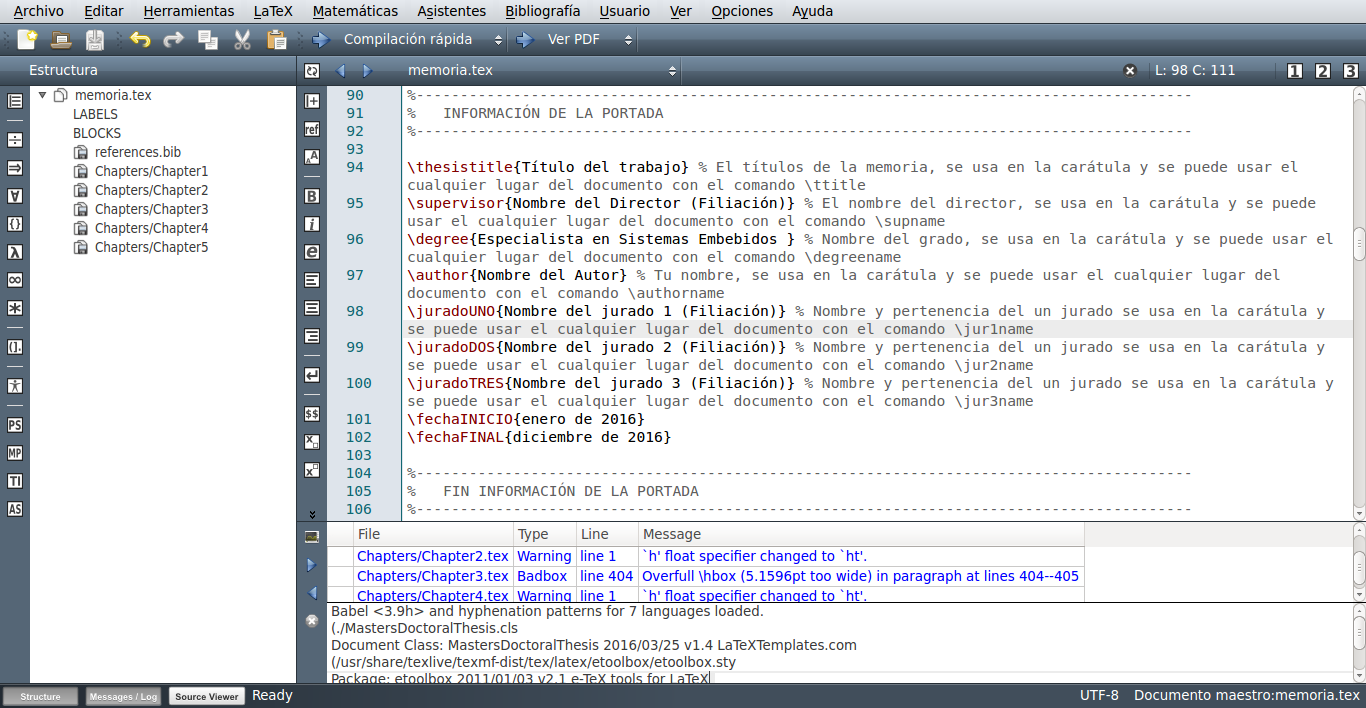
\includegraphics[width=.5\textwidth]{./Figures/texmaker.png}
	\caption{Entorno de trabajo de texMaker.}
	\label{fig:texmaker}
\end{figure}

\vspace{1cm}

Notar que existe una vista llamada Estructura a la izquierda de la interfaz que nos permite abrir desde dentro del programa los archivos individuales de los capítulos.  A la derecha se encuentra una vista con el archivo propiamente dicho para su edición. Hacia la parte inferior se encuentra una vista del log con información de los resultados de la compilación.  En esta última vista pueden aparecen advertencias o \textit{warning}, que normalmente pueden ser ignorados, y los errores que se indican en color rojo y deben resolverse para que se genere el PDF de salida.

Recordar que el archivo que se debe compilar con PDFLaTeX es \file{memoria.tex}, si se tratara de compilar alguno de los capítulos saldría un error.  Para salvar la molestia de tener que cambiar de archivo para compilar cada vez que se realice una modificación en un capítulo, se puede definir el archivo \file{memoria.tex} como ``documento maestro'' yendo al menú opciones -> ``definir documento actual como documento maestro'', lo que permite compilar con PDFLaTeX memoria.tex directamente desde cualquier archivo que se esté modificando . Se muestra esta opción en la figura \ref{fig:docMaestro}.

\begin{figure}[h]
	\centering
	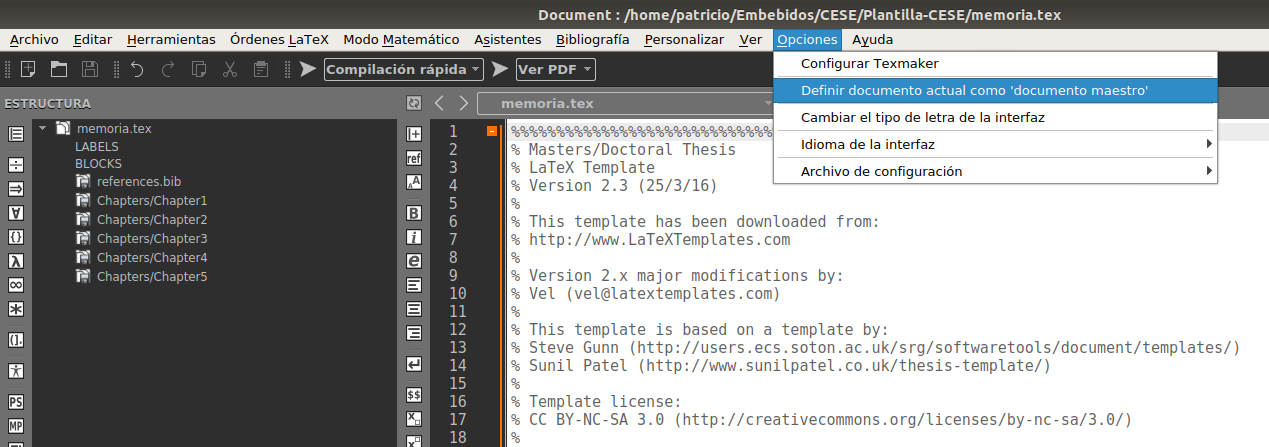
\includegraphics[width=\textwidth]{./Figures/docMaestro.png}
	\caption{Definir memoria.tex como documento maestro.}
	\label{fig:docMaestro}
\end{figure}

En el menú herramientas se encuentran las opciones de compilación.  Para producir un archivo PDF a partir de un archivo .tex se debe ejecutar PDFLaTeX (el shortcut es F6). Para incorporar nueva bibliografía se debe utilizar la opción BibTeX del mismo menú herramientas (el shortcut es F11).

Notar que para actualizar las tablas de contenidos se debe ejecutar PDFLaTeX dos veces.  Esto se debe a que es necesario actualizar algunos archivos auxiliares antes de obtener el resultado final.  En forma similar, para actualizar las referencias bibliográficas se debe ejecutar primero PDFLaTeX, después BibTeX y finalmente PDFLaTeX dos veces por idénticos motivos.

\section{Personalizando la plantilla, el archivo \file{memoria.tex}}
\label{sec:FillingFile}

Para personalizar la plantilla se debe incorporar la información propia en los distintos archivos \file{.tex}. 

Primero abrir \file{memoria.tex} con TexMaker (o el editor de su preferencia). Se debe ubicar dentro del archivo el bloque de código titulado \emph{INFORMACIÓN DE LA PORTADA} donde se deben incorporar los primeros datos personales con los que se construirá automáticamente la portada.


%----------------------------------------------------------------------------------------

\section{El código del archivo \file{memoria.tex} explicado}

El archivo \file{memoria.tex} contiene la estructura del documento y es el archivo de mayor jerarquía de la memoria.  Podría ser equiparable a la función \emph{main()} de un programa en C, o mejor dicho al archivo fuente .c donde se encuentra definida la función main().

La estructura básica de cualquier documento de \LaTeX{} comienza con la definición de clase del documento, es seguida por un preámbulo donde se pueden agregar funcionalidades con el uso de \texttt{paquetes} (equiparables a bibliotecas de C), y finalmente, termina con el cuerpo del documento, donde irá el contenido de la memoria.

\lstset{%
  basicstyle=\small\ttfamily,
  language=[LaTeX]{TeX}
}

\begin{lstlisting}
\documentclass{article}  <- Definicion de clase
\usepackage{listings}	 <- Preambulo

\begin{document}	 <- Comienzo del contenido propio 
	Hello world!
\end{document}
\end{lstlisting}


El archivo \file{memoria.tex} se encuentra densamente comentado para explicar qué páginas, secciones y elementos de formato está creando el código \LaTeX{} en cada línea. El código está dividido en bloques con nombres en mayúsculas para que resulte evidente qué es lo que hace esa porción de código en particular. Inicialmente puede parecer que hay mucho código \LaTeX{}, pero es principalmente código para dar formato a la memoria por lo que no requiere intervención del usuario de la plantilla.  Sí se deben personalizar con su información los bloques indicados como:

\begin{itemize}
	\item Informacion de la memoria
	\item Resumen
	\item Agradecimientos
	\item Dedicatoria
\end{itemize}

El índice de contenidos, las listas de figura de tablas se generan en forma automática y no requieren intervención ni edición manual por parte del usuario de la plantilla. 

En la parte final del documento se encuentran los capítulos y los apéndices.  Por defecto se incluyen los 5 capítulos propuestos que se encuentran en la carpeta /Chapters. Cada capítulo se debe escribir en un archivo .tex separado y se debe poner en la carpeta \emph{Chapters} con el nombre \file{Chapter1}, \file{Chapter2}, etc\ldots El código para incluir capítulos desde archivos externos se muestra a continuación.

\begin{verbatim}
	% Chapter 1

\chapter{Introducción general} % Main chapter title

\label{Chapter1} % For referencing the chapter elsewhere, use \ref{Chapter1} 
\label{IntroGeneral}

%----------------------------------------------------------------------------------------

% Define some commands to keep the formatting separated from the content 
\newcommand{\keyword}[1]{\textbf{#1}}
\newcommand{\tabhead}[1]{\textbf{#1}}
\newcommand{\code}[1]{\texttt{#1}}
\newcommand{\file}[1]{\texttt{\bfseries#1}}
\newcommand{\option}[1]{\texttt{\itshape#1}}
\newcommand{\grados}{$^{\circ}$}

%----------------------------------------------------------------------------------------

%\section{Introducción}

%----------------------------------------------------------------------------------------
\section{Aprendiendo \LaTeX{}}

\LaTeX{} no es \textsc{WYSIWYG} (What You See is What You Get), a diferencia de los procesadores de texto como Microsoft Word o Pages de Apple o incluso LibreOffice en el mundo open-source. En lugar de ello, un documento escrito para \LaTeX{} es en realidad un archivo de texto simple o llano que \emph{no contiene formato} . Nosotros le decimos a \LaTeX{} cómo deseamos que se aplique el formato en el documento final escribiendo comandos simples entre el texto, por ejemplo, si quiero usar texto en itálicas para dar énfasis, escribo \verb|\it{texto}| y pongo el texto que quiero en itálicas entre medio de las llaves. Esto significa que \LaTeX{} es un lenguaje del tipo \enquote{mark-up}, muy parecido a HTML.

\subsection{Una introducción (no tan corta) a \LaTeX{}}

Si sos nuevo en \LaTeX{}, hay un muy buen libro electrónico - disponible gratuitamente en Internet como un archivo PDF - llamado, \enquote{A (not so short) Introduction to \LaTeX{}}. El título del libro es generalmente acortado a simplemente \emph{lshort}. Puede descargar la versión más reciente en inglés (ya que se actualiza de vez en cuando) desde aquí:
\url{http://www.ctan.org/tex-archive/info/lshort/english/lshort.pdf}

Se puede encontrar la versión en español en la lista en esta página: \url{http://www.ctan.org/tex-archive/info/lshort/}

\subsubsection{Una subsubsección}

Acá tiene un ejemplo de una ``subsubsección'' que es el cuarto nivel de ordenamiento del texto, después de capítulo, sección y subsección.  Como se puede ver, las subsubsecciones no van numeradas en el cuerpo del documento ni en el índice.  El formato está definido por la plantilla y no debe ser modificado.

\subsection{Guía matemática rápida para \LaTeX{}}

Si estás escribiendo un documento con mucho contenido matemático, entonces es posible que desees leer el documento de la AMS (American Mathematical Society) llamado, \enquote{A Short Math Guide for \LaTeX{}}. Se puede encontrar en línea en el siguiente link: \url{http://www.ams.org/tex/amslatex.html} en la sección \enquote{Additional Documentation} hacia la parte inferior de la página.


%----------------------------------------------------------------------------------------

\section{Utilizando esta plantilla}

Si estás familiarizado con \LaTeX{}, entonces podés explorar la estructura de directorios de esta plantilla y proceder a personalizarla agregando tu información en el bloque \emph{INFORMACIÓN DE LA PORTADA} en el archivo \file{memoria.tex}.  

Se puede continuar luego modificando el resto de los archivos siguiendo los lineamientos que se describen en la sección \ref{sec:FillingFile} en la página \pageref{sec:FillingFile}.

Debés asegurarte de leer el capítulo \ref{Chapter2} acerca de las convenciones utilizadas para las Memoria de los Trabajos Finales de la \degreename.

Si sos nuevo en \LaTeX{}, se recomienda que continúes leyendo el documento ya que contiene información básica para aprovechar el potencial de esta herramienta.


%----------------------------------------------------------------------------------------

\section{Qué incluye esta plantilla}

\subsection{Carpetas}

Esta plantilla se distribuye como una único archivo .zip que se puede descomprimir en varios archivos y carpetas. Asimismo, se puede consultar el repositorio git para obtener la última versión de los archivos, \url{https://github.com/patriciobos/Plantilla-CESE.git}. Los nombres de las carpetas son, o pretender ser, auto-explicativos.

\keyword{Appendices} -- Esta es la carpeta donde se deben poner los apéndices. Cada apéndice debe ir en su propio archivo \file{.tex}. Se incluye un ejemplo y una plantilla en la carpeta.

\keyword{Chapters} -- Esta es la carpeta donde se deben poner los capítulos de la memoria. Cada capítulo debe ir un su propio archivo \file{.tex} por separado.  Se ofrece por defecto, la siguiente estructura de capítulos y se recomienda su utilización dentro de lo posible:

\begin{itemize}
\item Capítulo 1: Introducción general	
\item Capítulo 2: Introducción específica
\item Capítulo 3: Diseño e implementación
\item Capítulo 4: Ensayos y resultados
\item Capítulo 5: Conclusiones

\end{itemize}

Esta estructura de capítulos es la que se recomienda para las memorias de la especialización.

\keyword{Figures} -- Esta carpeta contiene todas las figuras de la memoria.  Estas son las versiones finales de las imágenes que van a ser incluidas en la memoria.  Pueden ser imágenes en formato \textit{raster}\footnote{\url{https://en.wikipedia.org/wiki/Raster_graphics}} como \file{.png}, \file{.jpg} o en formato vectoriales\footnote{\url{https://en.wikipedia.org/wiki/Vector_graphics}} como \file{.pdf}, \file{.ps}.  Se debe notar que utilizar imágenes vectoriales disminuye notablemente el peso del documento final y acelera el tiempo de compilación por lo que es recomendable su utilización siempre que sea posible.

\subsection{Archivos}

También están incluidos varios archivos, la mayoría de ellos son de texto plano y se puede ver su contenido en un editor de texto. Después de la compilación inicial, se verá que más archivos auxiliares son creados por \ LaTeX{} o BibTeX, pero son de uso interno y no es necesario hacer nada en particular con ellos.  Toda la información necesaria para compilar el documento se encuentra en los archivos \file{.tex}, \file{.bib}, \file{.cls} y en las imágenes de la carpeta Figures.

\keyword{referencias.bib} - este es un archivo importante que contiene toda la información de referencias bibliográficas que se utilizarán para las citas en la memoria en conjunto con BibTeX. Usted puede escribir las entradas bibliográficas en forma manual, aunque existen también programas de gestión de referencias que facilitan la creación y gestión de las referencias y permiten exportarlas en formato BibTeX.  También hay disponibles sitios web como \url{books.google.com} que permiten obtener toda la información necesaria para una cita en formato BibTeX. Ver sección \ref{sec:biblio}

\keyword{MastersDoctoralThesis.cls} -- este es un archivo importante. Es el archivos con la clase que le informa a \LaTeX{} cómo debe dar formato a la memoria. El usuario de la plantilla no debería necesitar modificar nada de este archivo.

\keyword{memoria.pdf} -- esta es su memoria con una tipografía bellamente compuesta (en formato de archivo PDF) creado por \LaTeX{}. Se distribuye con la plantilla y después de compilar por primera vez sin hacer ningún cambio se debería obtener una versión idéntica a este documento.

\keyword{memoria.tex} -- este es un archivo importante. Este es el archivo que tiene que compilar \LaTeX{} para producir la memoria como un archivo PDF. Contiene un marco de trabajo y estructuras que le indican a \LaTeX{} cómo diagramar la memoria.  Está altamente comentado para que se pueda entender qué es lo que realiza cada línea de código y por qué está incluida en ese lugar.  En este archivo se debe completar la información personalizada de las primeras sección según se indica en la sección \ref{sec:FillingFile}.

Archivos que \emph{no} forman parte de la distribución de la plantilla pero que son generados por \LaTeX{} como archivos auxiliares necesarios para la producción de la memoria.pdf son:

\keyword{memoria.aux} -- este es un archivo auxiliar generado por \LaTeX{}, si se borra \LaTeX{} simplemente lo regenera cuando se compila el archivo principal \file{memoria.tex}.

\keyword{memoria.bbl} -- este es un archivo auxiliar generado por BibTeX, si se borra BibTeX simplemente lo regenera cuando se compila el archivo principal \file{memoria.tex}. Mientras que el archivo \file{.bib} contiene todas las referencias que hay, este archivo \file{.bbl} contine sólo las referencias que han sido citadas y se utiliza para la construcción de la bibiografía.

\keyword{memoria.blg} -- este es un archivo auxiliar generado por BibTeX, si se borra BibTeX simplemente lo regenera cuando se compila el archivo principal \file{memoria.tex}.

\keyword{memoria.lof} -- este es un archivo auxiliar generado por \LaTeX{}, si se borra \LaTeX{} simplemente lo regenera cuando se compila el archivo principal \file{memoria.tex}.  Le indica a \LaTeX{} cómo construir la sección \emph{Lista de Figuras}.
 
\keyword{memoria.log} --  este es un archivo auxiliar generado por \LaTeX{}, si se borra \LaTeX{} simplemente lo regenera cuando se compila el archivo principal \file{memoria.tex}. Contiene mensajes de \LaTeX{}. Si se reciben errores o advertencias durante la compilación, se guardan en este archivo \file{.log}.

\keyword{memoria.lot} -- este es un archivo auxiliar generado por \LaTeX{}, si se borra \LaTeX{} simplemente lo regenera cuando se compila el archivo principal \file{memoria.tex}.  Le indica a \LaTeX{} cómo construir la sección \emph{Lista de Tablas}.

\keyword{memoria.out} -- este es un archivo auxiliar generado por \LaTeX{}, si se borra \LaTeX{} simplemente lo regenera cuando se compila el archivo principal \file{memoria.tex}.

De esta larga lista de archivos, sólo aquellos con la extensión \file{.bib}, \file{.cls} y \file{.tex} son importantes.  Los otros archivos auxiliares pueden ser ignorados o borrados ya que \LaTeX{} y BibTeX los regenerarán durante la compilación.

%----------------------------------------------------------------------------------------

\section{Entorno de trabajo}

Ante de comenzar a editar la plantilla debemos tener un editor \LaTeX{} instalado en nuestra computadora.  En forma análoga a lo que sucede en lenguaje C, que se puede crear y editar código con casi cualquier editor, existen ciertos entornos de trabajo que nos pueden simplificar mucho la tarea.  En este sentido, se recomienda, sobre todo para los principiantes en \LaTeX{} la utilización de TexMaker, un programa gratuito y multi-plantaforma que está disponible tanto para windows como para sistemas GNU/linux.

La versión más reciente de TexMaker es la 4.5 y se puede descargar del siguiente link: \url{http://www.xm1math.net/texmaker/download.html}. Se puede consultar el manual de usuario en el siguiente link: \url{http://www.xm1math.net/texmaker/doc.html}.
 

\subsection{Paquetes adicionales}

Si bien durante el proceso de instalación de TexMaker, o cualquier otro editor que se haya elegido, se instalarán en el sistema los paquetes básicos necesarios para trabajar con \LaTeX{}, la plantilla de los trabajos de Especialización y Maestría requieren de paquete adicionales.

Se indican a continuación los comandos que se deben introducir en la consola de Ubuntu (ctrl + alt + t) para instalarlos:

\begin{lstlisting}[language=bash]
  $ sudo apt install texlive-lang-spanish texlive-science 
  $ sudo apt install texlive-bibtex-extra biber
  $ sudo apt install texlive texlive-fonts-recommended
  $ sudo apt install texlive-latex-extra
\end{lstlisting}


\subsection{Configurando TexMaker}
\label{subsec:configurando}



Una vez instalado el programa y los paquetes adicionales se debe abrir el archivo memoria.tex con el editor para ver una pantalla similar a la que se puede apreciar en la figura \ref{fig:texmaker}. 
Una vez instalado el programa y los paquetes adicionales se debe abrir el archivo memoria.tex con el editor para ver una pantalla similar a la que se puede apreciar en la figura \ref{fig:texmaker}. 
Una vez instalado el programa y los paquetes adicionales se debe abrir el archivo memoria.tex con el editor para ver una pantalla similar a la que se puede apreciar en la figura \ref{fig:texmaker}. 
Una vez instalado el programa y los paquetes adicionales se debe abrir el archivo memoria.tex con el editor para ver una pantalla similar a la que se puede apreciar en la figura \ref{fig:texmaker}. 

\vspace{1cm}

\begin{figure}[htbp]
	\centering
	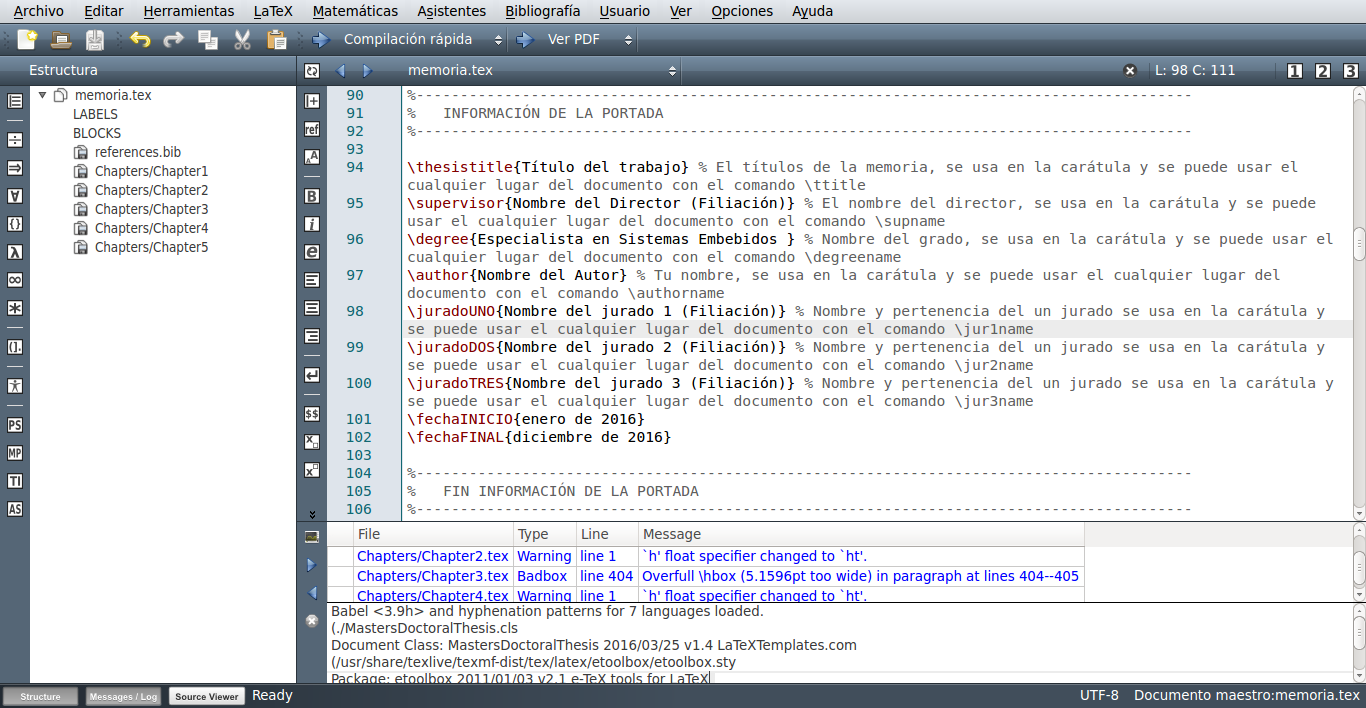
\includegraphics[width=.5\textwidth]{./Figures/texmaker.png}
	\caption{Entorno de trabajo de texMaker.}
	\label{fig:texmaker}
\end{figure}

\vspace{1cm}

Notar que existe una vista llamada Estructura a la izquierda de la interfaz que nos permite abrir desde dentro del programa los archivos individuales de los capítulos.  A la derecha se encuentra una vista con el archivo propiamente dicho para su edición. Hacia la parte inferior se encuentra una vista del log con información de los resultados de la compilación.  En esta última vista pueden aparecen advertencias o \textit{warning}, que normalmente pueden ser ignorados, y los errores que se indican en color rojo y deben resolverse para que se genere el PDF de salida.

Recordar que el archivo que se debe compilar con PDFLaTeX es \file{memoria.tex}, si se tratara de compilar alguno de los capítulos saldría un error.  Para salvar la molestia de tener que cambiar de archivo para compilar cada vez que se realice una modificación en un capítulo, se puede definir el archivo \file{memoria.tex} como ``documento maestro'' yendo al menú opciones -> ``definir documento actual como documento maestro'', lo que permite compilar con PDFLaTeX memoria.tex directamente desde cualquier archivo que se esté modificando . Se muestra esta opción en la figura \ref{fig:docMaestro}.

\begin{figure}[h]
	\centering
	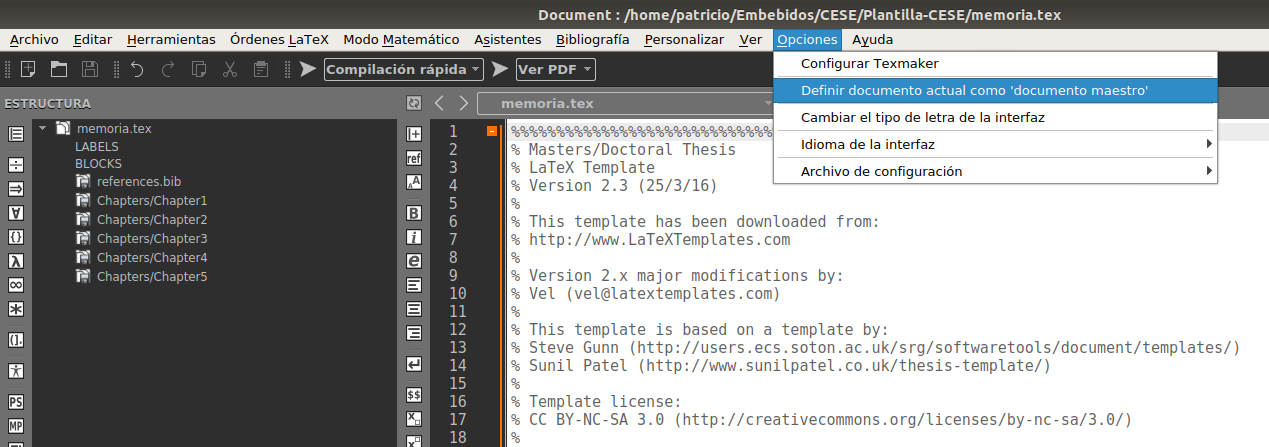
\includegraphics[width=\textwidth]{./Figures/docMaestro.png}
	\caption{Definir memoria.tex como documento maestro.}
	\label{fig:docMaestro}
\end{figure}

En el menú herramientas se encuentran las opciones de compilación.  Para producir un archivo PDF a partir de un archivo .tex se debe ejecutar PDFLaTeX (el shortcut es F6). Para incorporar nueva bibliografía se debe utilizar la opción BibTeX del mismo menú herramientas (el shortcut es F11).

Notar que para actualizar las tablas de contenidos se debe ejecutar PDFLaTeX dos veces.  Esto se debe a que es necesario actualizar algunos archivos auxiliares antes de obtener el resultado final.  En forma similar, para actualizar las referencias bibliográficas se debe ejecutar primero PDFLaTeX, después BibTeX y finalmente PDFLaTeX dos veces por idénticos motivos.

\section{Personalizando la plantilla, el archivo \file{memoria.tex}}
\label{sec:FillingFile}

Para personalizar la plantilla se debe incorporar la información propia en los distintos archivos \file{.tex}. 

Primero abrir \file{memoria.tex} con TexMaker (o el editor de su preferencia). Se debe ubicar dentro del archivo el bloque de código titulado \emph{INFORMACIÓN DE LA PORTADA} donde se deben incorporar los primeros datos personales con los que se construirá automáticamente la portada.


%----------------------------------------------------------------------------------------

\section{El código del archivo \file{memoria.tex} explicado}

El archivo \file{memoria.tex} contiene la estructura del documento y es el archivo de mayor jerarquía de la memoria.  Podría ser equiparable a la función \emph{main()} de un programa en C, o mejor dicho al archivo fuente .c donde se encuentra definida la función main().

La estructura básica de cualquier documento de \LaTeX{} comienza con la definición de clase del documento, es seguida por un preámbulo donde se pueden agregar funcionalidades con el uso de \texttt{paquetes} (equiparables a bibliotecas de C), y finalmente, termina con el cuerpo del documento, donde irá el contenido de la memoria.

\lstset{%
  basicstyle=\small\ttfamily,
  language=[LaTeX]{TeX}
}

\begin{lstlisting}
\documentclass{article}  <- Definicion de clase
\usepackage{listings}	 <- Preambulo

\begin{document}	 <- Comienzo del contenido propio 
	Hello world!
\end{document}
\end{lstlisting}


El archivo \file{memoria.tex} se encuentra densamente comentado para explicar qué páginas, secciones y elementos de formato está creando el código \LaTeX{} en cada línea. El código está dividido en bloques con nombres en mayúsculas para que resulte evidente qué es lo que hace esa porción de código en particular. Inicialmente puede parecer que hay mucho código \LaTeX{}, pero es principalmente código para dar formato a la memoria por lo que no requiere intervención del usuario de la plantilla.  Sí se deben personalizar con su información los bloques indicados como:

\begin{itemize}
	\item Informacion de la memoria
	\item Resumen
	\item Agradecimientos
	\item Dedicatoria
\end{itemize}

El índice de contenidos, las listas de figura de tablas se generan en forma automática y no requieren intervención ni edición manual por parte del usuario de la plantilla. 

En la parte final del documento se encuentran los capítulos y los apéndices.  Por defecto se incluyen los 5 capítulos propuestos que se encuentran en la carpeta /Chapters. Cada capítulo se debe escribir en un archivo .tex separado y se debe poner en la carpeta \emph{Chapters} con el nombre \file{Chapter1}, \file{Chapter2}, etc\ldots El código para incluir capítulos desde archivos externos se muestra a continuación.

\begin{verbatim}
	% Chapter 1

\chapter{Introducción general} % Main chapter title

\label{Chapter1} % For referencing the chapter elsewhere, use \ref{Chapter1} 
\label{IntroGeneral}

%----------------------------------------------------------------------------------------

% Define some commands to keep the formatting separated from the content 
\newcommand{\keyword}[1]{\textbf{#1}}
\newcommand{\tabhead}[1]{\textbf{#1}}
\newcommand{\code}[1]{\texttt{#1}}
\newcommand{\file}[1]{\texttt{\bfseries#1}}
\newcommand{\option}[1]{\texttt{\itshape#1}}
\newcommand{\grados}{$^{\circ}$}

%----------------------------------------------------------------------------------------

%\section{Introducción}

%----------------------------------------------------------------------------------------
\section{Aprendiendo \LaTeX{}}

\LaTeX{} no es \textsc{WYSIWYG} (What You See is What You Get), a diferencia de los procesadores de texto como Microsoft Word o Pages de Apple o incluso LibreOffice en el mundo open-source. En lugar de ello, un documento escrito para \LaTeX{} es en realidad un archivo de texto simple o llano que \emph{no contiene formato} . Nosotros le decimos a \LaTeX{} cómo deseamos que se aplique el formato en el documento final escribiendo comandos simples entre el texto, por ejemplo, si quiero usar texto en itálicas para dar énfasis, escribo \verb|\it{texto}| y pongo el texto que quiero en itálicas entre medio de las llaves. Esto significa que \LaTeX{} es un lenguaje del tipo \enquote{mark-up}, muy parecido a HTML.

\subsection{Una introducción (no tan corta) a \LaTeX{}}

Si sos nuevo en \LaTeX{}, hay un muy buen libro electrónico - disponible gratuitamente en Internet como un archivo PDF - llamado, \enquote{A (not so short) Introduction to \LaTeX{}}. El título del libro es generalmente acortado a simplemente \emph{lshort}. Puede descargar la versión más reciente en inglés (ya que se actualiza de vez en cuando) desde aquí:
\url{http://www.ctan.org/tex-archive/info/lshort/english/lshort.pdf}

Se puede encontrar la versión en español en la lista en esta página: \url{http://www.ctan.org/tex-archive/info/lshort/}

\subsubsection{Una subsubsección}

Acá tiene un ejemplo de una ``subsubsección'' que es el cuarto nivel de ordenamiento del texto, después de capítulo, sección y subsección.  Como se puede ver, las subsubsecciones no van numeradas en el cuerpo del documento ni en el índice.  El formato está definido por la plantilla y no debe ser modificado.

\subsection{Guía matemática rápida para \LaTeX{}}

Si estás escribiendo un documento con mucho contenido matemático, entonces es posible que desees leer el documento de la AMS (American Mathematical Society) llamado, \enquote{A Short Math Guide for \LaTeX{}}. Se puede encontrar en línea en el siguiente link: \url{http://www.ams.org/tex/amslatex.html} en la sección \enquote{Additional Documentation} hacia la parte inferior de la página.


%----------------------------------------------------------------------------------------

\section{Utilizando esta plantilla}

Si estás familiarizado con \LaTeX{}, entonces podés explorar la estructura de directorios de esta plantilla y proceder a personalizarla agregando tu información en el bloque \emph{INFORMACIÓN DE LA PORTADA} en el archivo \file{memoria.tex}.  

Se puede continuar luego modificando el resto de los archivos siguiendo los lineamientos que se describen en la sección \ref{sec:FillingFile} en la página \pageref{sec:FillingFile}.

Debés asegurarte de leer el capítulo \ref{Chapter2} acerca de las convenciones utilizadas para las Memoria de los Trabajos Finales de la \degreename.

Si sos nuevo en \LaTeX{}, se recomienda que continúes leyendo el documento ya que contiene información básica para aprovechar el potencial de esta herramienta.


%----------------------------------------------------------------------------------------

\section{Qué incluye esta plantilla}

\subsection{Carpetas}

Esta plantilla se distribuye como una único archivo .zip que se puede descomprimir en varios archivos y carpetas. Asimismo, se puede consultar el repositorio git para obtener la última versión de los archivos, \url{https://github.com/patriciobos/Plantilla-CESE.git}. Los nombres de las carpetas son, o pretender ser, auto-explicativos.

\keyword{Appendices} -- Esta es la carpeta donde se deben poner los apéndices. Cada apéndice debe ir en su propio archivo \file{.tex}. Se incluye un ejemplo y una plantilla en la carpeta.

\keyword{Chapters} -- Esta es la carpeta donde se deben poner los capítulos de la memoria. Cada capítulo debe ir un su propio archivo \file{.tex} por separado.  Se ofrece por defecto, la siguiente estructura de capítulos y se recomienda su utilización dentro de lo posible:

\begin{itemize}
\item Capítulo 1: Introducción general	
\item Capítulo 2: Introducción específica
\item Capítulo 3: Diseño e implementación
\item Capítulo 4: Ensayos y resultados
\item Capítulo 5: Conclusiones

\end{itemize}

Esta estructura de capítulos es la que se recomienda para las memorias de la especialización.

\keyword{Figures} -- Esta carpeta contiene todas las figuras de la memoria.  Estas son las versiones finales de las imágenes que van a ser incluidas en la memoria.  Pueden ser imágenes en formato \textit{raster}\footnote{\url{https://en.wikipedia.org/wiki/Raster_graphics}} como \file{.png}, \file{.jpg} o en formato vectoriales\footnote{\url{https://en.wikipedia.org/wiki/Vector_graphics}} como \file{.pdf}, \file{.ps}.  Se debe notar que utilizar imágenes vectoriales disminuye notablemente el peso del documento final y acelera el tiempo de compilación por lo que es recomendable su utilización siempre que sea posible.

\subsection{Archivos}

También están incluidos varios archivos, la mayoría de ellos son de texto plano y se puede ver su contenido en un editor de texto. Después de la compilación inicial, se verá que más archivos auxiliares son creados por \ LaTeX{} o BibTeX, pero son de uso interno y no es necesario hacer nada en particular con ellos.  Toda la información necesaria para compilar el documento se encuentra en los archivos \file{.tex}, \file{.bib}, \file{.cls} y en las imágenes de la carpeta Figures.

\keyword{referencias.bib} - este es un archivo importante que contiene toda la información de referencias bibliográficas que se utilizarán para las citas en la memoria en conjunto con BibTeX. Usted puede escribir las entradas bibliográficas en forma manual, aunque existen también programas de gestión de referencias que facilitan la creación y gestión de las referencias y permiten exportarlas en formato BibTeX.  También hay disponibles sitios web como \url{books.google.com} que permiten obtener toda la información necesaria para una cita en formato BibTeX. Ver sección \ref{sec:biblio}

\keyword{MastersDoctoralThesis.cls} -- este es un archivo importante. Es el archivos con la clase que le informa a \LaTeX{} cómo debe dar formato a la memoria. El usuario de la plantilla no debería necesitar modificar nada de este archivo.

\keyword{memoria.pdf} -- esta es su memoria con una tipografía bellamente compuesta (en formato de archivo PDF) creado por \LaTeX{}. Se distribuye con la plantilla y después de compilar por primera vez sin hacer ningún cambio se debería obtener una versión idéntica a este documento.

\keyword{memoria.tex} -- este es un archivo importante. Este es el archivo que tiene que compilar \LaTeX{} para producir la memoria como un archivo PDF. Contiene un marco de trabajo y estructuras que le indican a \LaTeX{} cómo diagramar la memoria.  Está altamente comentado para que se pueda entender qué es lo que realiza cada línea de código y por qué está incluida en ese lugar.  En este archivo se debe completar la información personalizada de las primeras sección según se indica en la sección \ref{sec:FillingFile}.

Archivos que \emph{no} forman parte de la distribución de la plantilla pero que son generados por \LaTeX{} como archivos auxiliares necesarios para la producción de la memoria.pdf son:

\keyword{memoria.aux} -- este es un archivo auxiliar generado por \LaTeX{}, si se borra \LaTeX{} simplemente lo regenera cuando se compila el archivo principal \file{memoria.tex}.

\keyword{memoria.bbl} -- este es un archivo auxiliar generado por BibTeX, si se borra BibTeX simplemente lo regenera cuando se compila el archivo principal \file{memoria.tex}. Mientras que el archivo \file{.bib} contiene todas las referencias que hay, este archivo \file{.bbl} contine sólo las referencias que han sido citadas y se utiliza para la construcción de la bibiografía.

\keyword{memoria.blg} -- este es un archivo auxiliar generado por BibTeX, si se borra BibTeX simplemente lo regenera cuando se compila el archivo principal \file{memoria.tex}.

\keyword{memoria.lof} -- este es un archivo auxiliar generado por \LaTeX{}, si se borra \LaTeX{} simplemente lo regenera cuando se compila el archivo principal \file{memoria.tex}.  Le indica a \LaTeX{} cómo construir la sección \emph{Lista de Figuras}.
 
\keyword{memoria.log} --  este es un archivo auxiliar generado por \LaTeX{}, si se borra \LaTeX{} simplemente lo regenera cuando se compila el archivo principal \file{memoria.tex}. Contiene mensajes de \LaTeX{}. Si se reciben errores o advertencias durante la compilación, se guardan en este archivo \file{.log}.

\keyword{memoria.lot} -- este es un archivo auxiliar generado por \LaTeX{}, si se borra \LaTeX{} simplemente lo regenera cuando se compila el archivo principal \file{memoria.tex}.  Le indica a \LaTeX{} cómo construir la sección \emph{Lista de Tablas}.

\keyword{memoria.out} -- este es un archivo auxiliar generado por \LaTeX{}, si se borra \LaTeX{} simplemente lo regenera cuando se compila el archivo principal \file{memoria.tex}.

De esta larga lista de archivos, sólo aquellos con la extensión \file{.bib}, \file{.cls} y \file{.tex} son importantes.  Los otros archivos auxiliares pueden ser ignorados o borrados ya que \LaTeX{} y BibTeX los regenerarán durante la compilación.

%----------------------------------------------------------------------------------------

\section{Entorno de trabajo}

Ante de comenzar a editar la plantilla debemos tener un editor \LaTeX{} instalado en nuestra computadora.  En forma análoga a lo que sucede en lenguaje C, que se puede crear y editar código con casi cualquier editor, existen ciertos entornos de trabajo que nos pueden simplificar mucho la tarea.  En este sentido, se recomienda, sobre todo para los principiantes en \LaTeX{} la utilización de TexMaker, un programa gratuito y multi-plantaforma que está disponible tanto para windows como para sistemas GNU/linux.

La versión más reciente de TexMaker es la 4.5 y se puede descargar del siguiente link: \url{http://www.xm1math.net/texmaker/download.html}. Se puede consultar el manual de usuario en el siguiente link: \url{http://www.xm1math.net/texmaker/doc.html}.
 

\subsection{Paquetes adicionales}

Si bien durante el proceso de instalación de TexMaker, o cualquier otro editor que se haya elegido, se instalarán en el sistema los paquetes básicos necesarios para trabajar con \LaTeX{}, la plantilla de los trabajos de Especialización y Maestría requieren de paquete adicionales.

Se indican a continuación los comandos que se deben introducir en la consola de Ubuntu (ctrl + alt + t) para instalarlos:

\begin{lstlisting}[language=bash]
  $ sudo apt install texlive-lang-spanish texlive-science 
  $ sudo apt install texlive-bibtex-extra biber
  $ sudo apt install texlive texlive-fonts-recommended
  $ sudo apt install texlive-latex-extra
\end{lstlisting}


\subsection{Configurando TexMaker}
\label{subsec:configurando}



Una vez instalado el programa y los paquetes adicionales se debe abrir el archivo memoria.tex con el editor para ver una pantalla similar a la que se puede apreciar en la figura \ref{fig:texmaker}. 
Una vez instalado el programa y los paquetes adicionales se debe abrir el archivo memoria.tex con el editor para ver una pantalla similar a la que se puede apreciar en la figura \ref{fig:texmaker}. 
Una vez instalado el programa y los paquetes adicionales se debe abrir el archivo memoria.tex con el editor para ver una pantalla similar a la que se puede apreciar en la figura \ref{fig:texmaker}. 
Una vez instalado el programa y los paquetes adicionales se debe abrir el archivo memoria.tex con el editor para ver una pantalla similar a la que se puede apreciar en la figura \ref{fig:texmaker}. 

\vspace{1cm}

\begin{figure}[htbp]
	\centering
	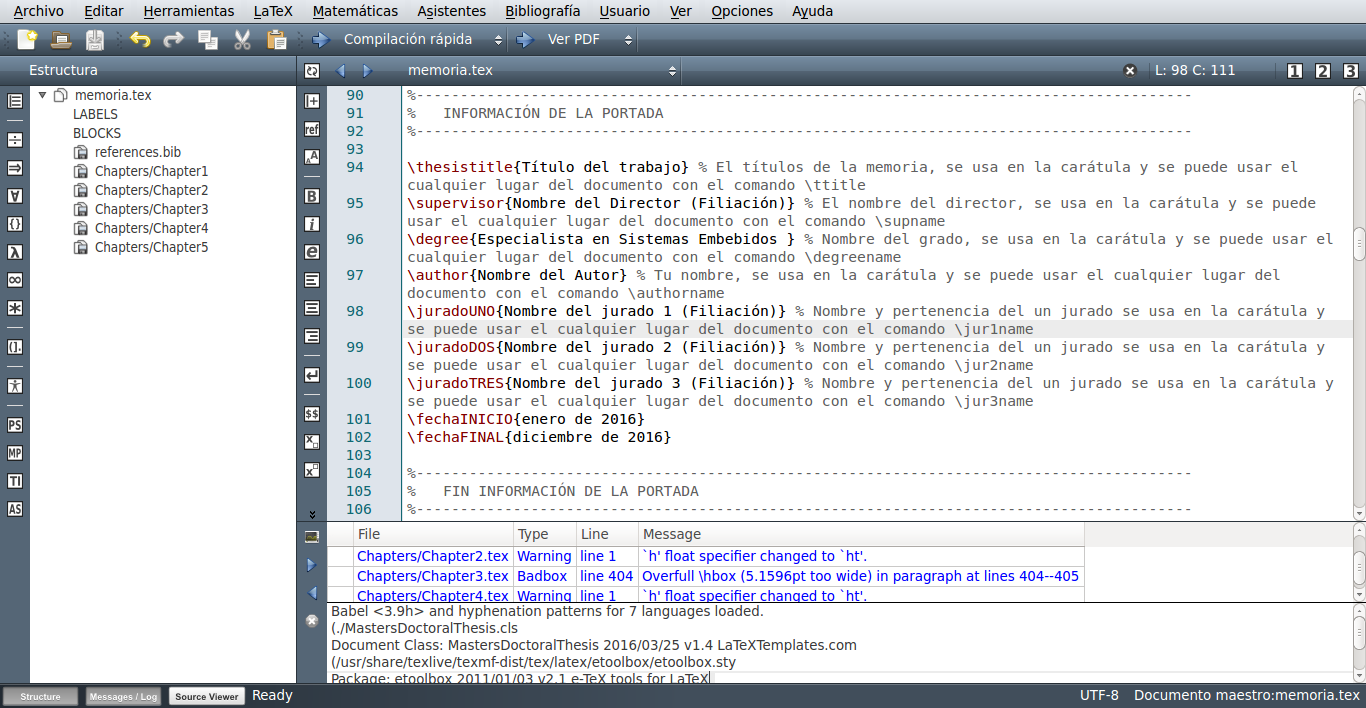
\includegraphics[width=.5\textwidth]{./Figures/texmaker.png}
	\caption{Entorno de trabajo de texMaker.}
	\label{fig:texmaker}
\end{figure}

\vspace{1cm}

Notar que existe una vista llamada Estructura a la izquierda de la interfaz que nos permite abrir desde dentro del programa los archivos individuales de los capítulos.  A la derecha se encuentra una vista con el archivo propiamente dicho para su edición. Hacia la parte inferior se encuentra una vista del log con información de los resultados de la compilación.  En esta última vista pueden aparecen advertencias o \textit{warning}, que normalmente pueden ser ignorados, y los errores que se indican en color rojo y deben resolverse para que se genere el PDF de salida.

Recordar que el archivo que se debe compilar con PDFLaTeX es \file{memoria.tex}, si se tratara de compilar alguno de los capítulos saldría un error.  Para salvar la molestia de tener que cambiar de archivo para compilar cada vez que se realice una modificación en un capítulo, se puede definir el archivo \file{memoria.tex} como ``documento maestro'' yendo al menú opciones -> ``definir documento actual como documento maestro'', lo que permite compilar con PDFLaTeX memoria.tex directamente desde cualquier archivo que se esté modificando . Se muestra esta opción en la figura \ref{fig:docMaestro}.

\begin{figure}[h]
	\centering
	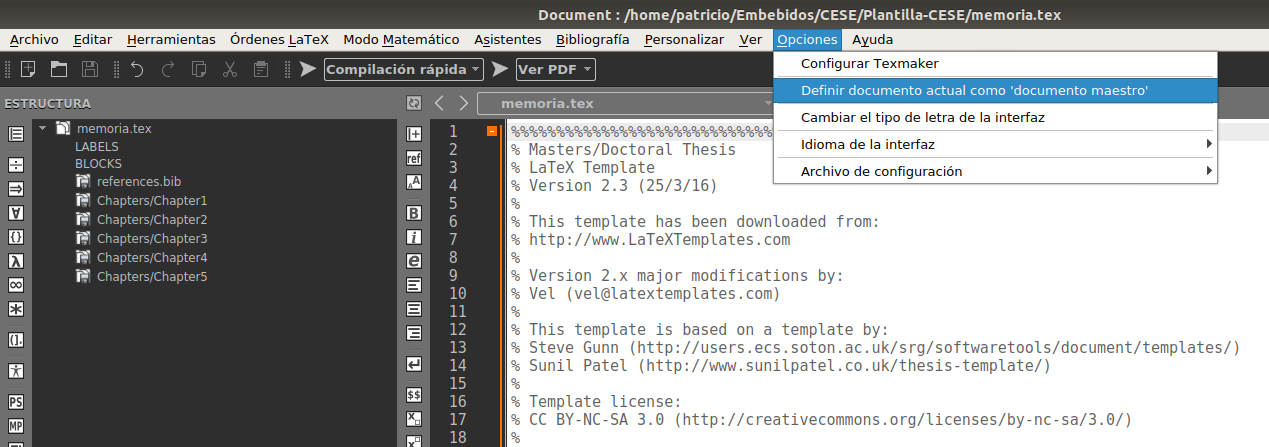
\includegraphics[width=\textwidth]{./Figures/docMaestro.png}
	\caption{Definir memoria.tex como documento maestro.}
	\label{fig:docMaestro}
\end{figure}

En el menú herramientas se encuentran las opciones de compilación.  Para producir un archivo PDF a partir de un archivo .tex se debe ejecutar PDFLaTeX (el shortcut es F6). Para incorporar nueva bibliografía se debe utilizar la opción BibTeX del mismo menú herramientas (el shortcut es F11).

Notar que para actualizar las tablas de contenidos se debe ejecutar PDFLaTeX dos veces.  Esto se debe a que es necesario actualizar algunos archivos auxiliares antes de obtener el resultado final.  En forma similar, para actualizar las referencias bibliográficas se debe ejecutar primero PDFLaTeX, después BibTeX y finalmente PDFLaTeX dos veces por idénticos motivos.

\section{Personalizando la plantilla, el archivo \file{memoria.tex}}
\label{sec:FillingFile}

Para personalizar la plantilla se debe incorporar la información propia en los distintos archivos \file{.tex}. 

Primero abrir \file{memoria.tex} con TexMaker (o el editor de su preferencia). Se debe ubicar dentro del archivo el bloque de código titulado \emph{INFORMACIÓN DE LA PORTADA} donde se deben incorporar los primeros datos personales con los que se construirá automáticamente la portada.


%----------------------------------------------------------------------------------------

\section{El código del archivo \file{memoria.tex} explicado}

El archivo \file{memoria.tex} contiene la estructura del documento y es el archivo de mayor jerarquía de la memoria.  Podría ser equiparable a la función \emph{main()} de un programa en C, o mejor dicho al archivo fuente .c donde se encuentra definida la función main().

La estructura básica de cualquier documento de \LaTeX{} comienza con la definición de clase del documento, es seguida por un preámbulo donde se pueden agregar funcionalidades con el uso de \texttt{paquetes} (equiparables a bibliotecas de C), y finalmente, termina con el cuerpo del documento, donde irá el contenido de la memoria.

\lstset{%
  basicstyle=\small\ttfamily,
  language=[LaTeX]{TeX}
}

\begin{lstlisting}
\documentclass{article}  <- Definicion de clase
\usepackage{listings}	 <- Preambulo

\begin{document}	 <- Comienzo del contenido propio 
	Hello world!
\end{document}
\end{lstlisting}


El archivo \file{memoria.tex} se encuentra densamente comentado para explicar qué páginas, secciones y elementos de formato está creando el código \LaTeX{} en cada línea. El código está dividido en bloques con nombres en mayúsculas para que resulte evidente qué es lo que hace esa porción de código en particular. Inicialmente puede parecer que hay mucho código \LaTeX{}, pero es principalmente código para dar formato a la memoria por lo que no requiere intervención del usuario de la plantilla.  Sí se deben personalizar con su información los bloques indicados como:

\begin{itemize}
	\item Informacion de la memoria
	\item Resumen
	\item Agradecimientos
	\item Dedicatoria
\end{itemize}

El índice de contenidos, las listas de figura de tablas se generan en forma automática y no requieren intervención ni edición manual por parte del usuario de la plantilla. 

En la parte final del documento se encuentran los capítulos y los apéndices.  Por defecto se incluyen los 5 capítulos propuestos que se encuentran en la carpeta /Chapters. Cada capítulo se debe escribir en un archivo .tex separado y se debe poner en la carpeta \emph{Chapters} con el nombre \file{Chapter1}, \file{Chapter2}, etc\ldots El código para incluir capítulos desde archivos externos se muestra a continuación.

\begin{verbatim}
	\include{Chapters/Chapter1}
	\include{Chapters/Chapter2} 
	\include{Chapters/Chapter3}
	\include{Chapters/Chapter4} 
	\include{Chapters/Chapter5} 
\end{verbatim}

Los apéndices también deben escribirse en archivos .tex separados, que se deben ubicar dentro de la carpeta \emph{Appendices}. Los apéndices vienen comentados por defecto con el caracter \code{\%} y para incluirlos simplemente se debe eliminar dicho caracter.

Finalmente, se encuentra el código para incluir la bibliografía en el documento final.  Este código tampoco debe modificarse. La metodología para trabajar las referencias bibliográficas se desarrolla en la sección \ref{sec:biblio}.
%----------------------------------------------------------------------------------------

\section{Bibliografía}
\label{sec:biblio}

Las opciones de formato de la bibliografía se controlan a través del paquete de latex \option{biblatex} que se incluye en la memoria en el archivo memoria.tex.  Estas opciones determinan cómo se generan las citas bibliográficas en el cuerpo del documento y cómo se genera la bibliografía al final de la memoria.

En el preámbulo se puede encontrar el código que incluye el paquete biblatex, que no requiere ninguna modificación del usuario de la plantilla, y que contiene las siguientes opciones:

\begin{lstlisting}
\usepackage[backend=bibtex,
	natbib=true, 
	style=numeric, 
	sorting=none]
{biblatex}
\end{lstlisting}

En el archivo \file{reference.bib} se encuentran las referencias bibliográficas que se pueden citar en el documento.  Para incorporar una nueva cita al documento lo primero es agregarla en este archivo con todos los campos necesario.  Todas las entradas bibliográficas comienzan con $@$ y una palabra que define el formato de la entrada.  Para cada formato existen campos obligatorios que deben completarse. No importa el orden en que las entradas estén definidas en el archivo .bib.  Tampoco es importante el orden en que estén definidos los campos de una entrada bibliográfica. A continuación se muestran algunos ejemplos:

\begin{lstlisting}
@ARTICLE{ARTICLE:1,
    AUTHOR="John Doe",
    TITLE="Title",
    JOURNAL="Journal",
    YEAR="2017",
}
\end{lstlisting}


\begin{lstlisting}
@BOOK{BOOK:1,
    AUTHOR="John Doe",
    TITLE="The Book without Title",
    PUBLISHER="Dummy Publisher",
    YEAR="2100",
}
\end{lstlisting}


\begin{lstlisting}
@INBOOK{BOOK:2,
    AUTHOR="John Doe",
    TITLE="The Book without Title",
    PUBLISHER="Dummy Publisher",
    YEAR="2100",
    PAGES="100-200",
}
\end{lstlisting}


\begin{lstlisting}
@MISC{WEBSITE:1,
    HOWPUBLISHED = "\url{http://example.com}",
    AUTHOR = "Intel",
    TITLE = "Example Website",
    MONTH = "12",
    YEAR = "1988",
    URLDATE = {2012-11-26}
}
\end{lstlisting}

Se debe notar que los nombres \emph{ARTICLE:1}, \emph{BOOK:1}, \emph{BOOK:2} y \emph{WEBSITE:1} son nombres de fantasía que le sirve al autor del documento para identificar la entrada. En este sentido, se podrían reemplazar por cualquier otro nombre.  Tampoco es necesario poner : seguido de un número, en los ejemplos sólo se incluye como un posible estilo para identificar las entradas.

La entradas se citan en el documento con el comando: 

\begin{verbatim}
\citep{nombre_de_la_entrada}
\end{verbatim}

Y cuando se usan, se muestran así: \citep{ARTICLE:1}, \citep{BOOK:1}, \citep{BOOK:2}, \citep{WEBSITE:1}.  Notar cómo se conforma la sección Bibliografía al final del documento.

Finalmente y como se mencionó en la subsección \ref{subsec:configurando}, para actualizar las referencias bibliográficas tanto en la sección bibliografía como las citas en el cuerpo del documento, se deben ejecutar las herramientas de compilación PDFLaTeX, BibTeX, PDFLaTeX, PDFLaTeX, en ese orden.  Este procedimiento debería resolver cualquier mensaje "Citation xxxxx on page x undefined".

	\chapter{Introducción específica} % Main chapter title

El presente capítulo describe los elementos componentes del sistema, el principio de funcionamiento y los requerimientos acordados con el cliente sobre el sistema.


\label{Chapter2}

%----------------------------------------------------------------------------------------
%	SECTION 1
%----------------------------------------------------------------------------------------


\section{Elementos componentes del sistema}
\label{sec:elementos_componentes_sistema}

Para entender el funcionamiento del sistema, es necesario conocer los elementos que lo componen. La presente sección describirá tanto los elementos físicos necesarios para conocer al sistema que se busca representar, como las herramientas de software utilizadas para el desarrollo del emulador.

\subsection{Elementos físicos del sistema}
\label{subsec:elementos_fisicos}

La presente sección dará una descripción general de los elementos que serán de vital importancia para el proyecto.

\subsubsection{Bootloader}
\label{subsec:bootloader}

El \textit{bootloader} es una pieza de software relativamente simple, cuyo principal objetivo es cargar el software de vuelo en la memoria RAM del sistema. Una vez cargado el software de vuelo, le cede el control al software de vuelo, el cual se encarga de ejecutar la misión del sistema.

En misiones espaciales es común que el \textit{bootloader} tenga la capacidad de verificar la integridad del software de vuelo antes de cargarlo en la memoria RAM, así mismo, de cargar diferentes versiones del software de vuelo en caso de que alguna de ellas se encuentre dañada.

\subsubsection{Firmware}
\label{subsec:firmware}

El \textit{firmware} es un software que se encuentra almacenado en la memoria no volátil del sistema, y es el encargado de inicializar los periféricos del sistema. Usualmente, este componente es desarrollado por un equipo especializado tanto en la misión para la que se está desarrollando el sistema, como en la arquitectura del microprocesador que se está utilizando. En el caso de aplicaciones espaciales, el \textit{firmware} es llamado software de vuelo o \textit{Fly Software} (FSW).

Normalmente, en la memoria no volátil del sistema se almacenan múltiples versiones del software de vuelo. Varias de ellas están presentes para servir de redundancia, en caso de que alguna de ellas se encuentre dañada, como para almacenar distintas versiones del software de vuelo con modos de operación más limitados pero seguros.

\subsubsection{Unidad de procesamiento}
\label{subsec:unidad_procesamiento}
Todo lo previamente mencionado se ejecuta en la unidad de procesamiento o CPU. La CPU es el componente encargado de ejecutar las instrucciones tanto del \textit{bootloader} como del software de vuelo.

El CPU interactúa con los periféricos del sistema, especialmente con la memoria RAM del sistema, ya que es el medio de almacenamiento masivo de alta velocidad de acceso.

El CPU, una vez encendido, empezará a leer las instrucciones de una posición dada por el fabricante y ejecutarlas secuencialmente. Es deber del desarrollador posicionar al \textit{bootloader} en esa posición de memoria.

\subsection{Software utilizado}
\label{subsec:software_utilizado}

La presente sección describirá las herramientas de software que fueron utilizadas para el desarrollo del trabajo.

\subsubsection{C++}
\label{subsec:cpp}

Dado que el emulador es un software que simula el comportamiento de un CPU, es necesario que el lenguaje de programación utilizado sea de bajo nivel, permitiendo mejores tiempos de ejecución y un mayor control sobre los recursos utilizados. Por lo tanto, se decidió utilizar C++ como lenguaje de programación para el desarrollo del emulador.

Otro motivo para su elección es que C++ es un lenguaje de programación ampliamente utilizado en la industria, por lo que facilita la comunicación con otros desarrolladores y la integración con otros sistemas.

\subsubsection{Herramientas Clang}
\label{subsec:clang_tidy}

Se utilizó Clang Tidy como herramienta de análisis estático de código. Permitiendo una mayor calidad del código y sintaxis uniforme. Así mismo se forzaron reglas para evitar malas prácticas comunes en los lenguajes de programación de bajo nivel, tales como el uso de memoria no inicializada, o aritmética de punteros.

También se utilizó Clang Format para mantener un estilo de código uniforme en todo el proyecto.

\subsubsection{Latex}
\label{subsec:latex}

Se utilizó Latex como herramienta de escritura de la documentación para el manual de usuario del proyecto. Dicha elección se tomo debido a que Latex es una herramienta ampliamente utilizada en la industria para la escritura de documentos técnicos.

El manual de usuario busca ser una guía completa y en detalle de la herramienta, no solo explicando la interfaz expuesta, sino decisiones de diseño y funcionamiento interno de la herramienta.

\subsubsection{Doxygen}
\label{subsec:doxygen}

Se utilizó Doxygen como herramienta de generación de documentación del código fuente. Con esta herramienta se generó un sitio web el cual describe la interfaz para interactuar con la herramienta (API). Dicha documentación busca ser una guía rápida para desarrolladores que estén utilizando el emulador.


\section{Principio de funcionamiento}
\label{sec:principio_funcionamiento}

El funcionamiento de un CPU, y por lo tanto de un emulador, se puede mostrar de manera simplificada de forma gráfica:

\begin{figure}[htbp]
	\centering
	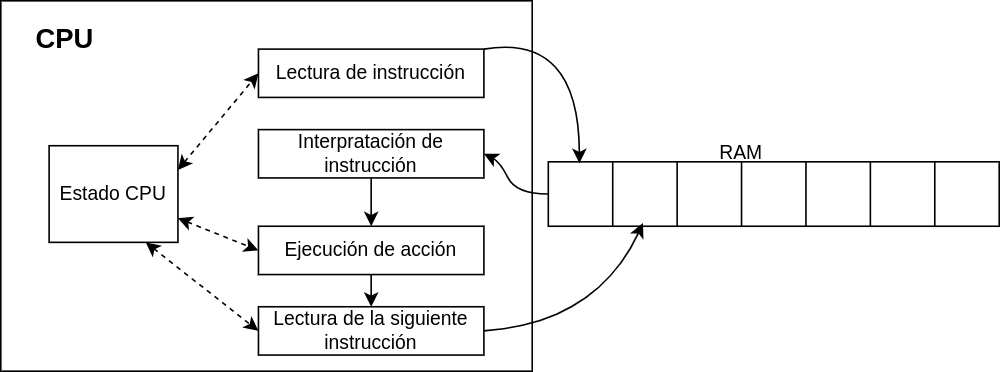
\includegraphics[width=1\textwidth]{./Figures/funcionamiento_emulador}
	\caption{Funcionamiento de alto nivel de un CPU o emulador.}
	\label{fig:functionamiento_emulador}
\end{figure}

Dicho flujo se ejecuta de manera continua, y no necesariamente las instrucciones se ejecutan en el orden en el que se encuentran en la memoria. Esto se debe a que el CPU tiene instrucciones de salto condicional, instrucciones de salto incondicional, y puede recibir interrupciones que cambien el flujo de ejecución del programa.


Un desafío que se tuvo que resolver temprana en el desarrollo del emulador fue la endianess del sistema. El endianess es el orden en el que se almacenan los bytes en la memoria. En el caso de la arquitectura SPARC V8, se utiliza el ordenamiento \textit{big-endian}, lo que significa que el byte más significativo se almacena en la dirección de memoria más alta. Por otro lado, la arquitectura x86 (Es decir, nuestros computadoras de escritorio) utiliza el ordenamiento \textit{little-endian}, donde el byte menos significativo se almacena en la dirección de memoria más baja. Por lo tanto, al momento de interpretar los datos obtenidos de la memoria, se debe reordenar los bytes para que tengan sentido. Dicha problemática es propia únicamente del emulado

\section{Requerimientos}
\label{sec:requerimientos}

 
	\chapter{Diseño e implementación} % Main chapter title
\label{Chapter3}

El presente capítulo describe los elementos componentes del sistema en detalle, las consideraciones y decisiones técnicas tomadas durante el desarrollo del emulador, el diagrama de bloques del sistema, la arquitectura del software y los módulos que lo componen.

%----------------------------------------------------------------------------------------
%	SECTION 1
%----------------------------------------------------------------------------------------


\section{Consideraciones y desiciones técnicas}
\label{sec:consideraciones_decisiones_tecnicas}

El trabajo realizado se puede dividir en cuatro grandes componentes, tal como se muestra en la figura \ref{fig:diagrama_bloques}:

\begin{figure}[htbp]
	\centering
	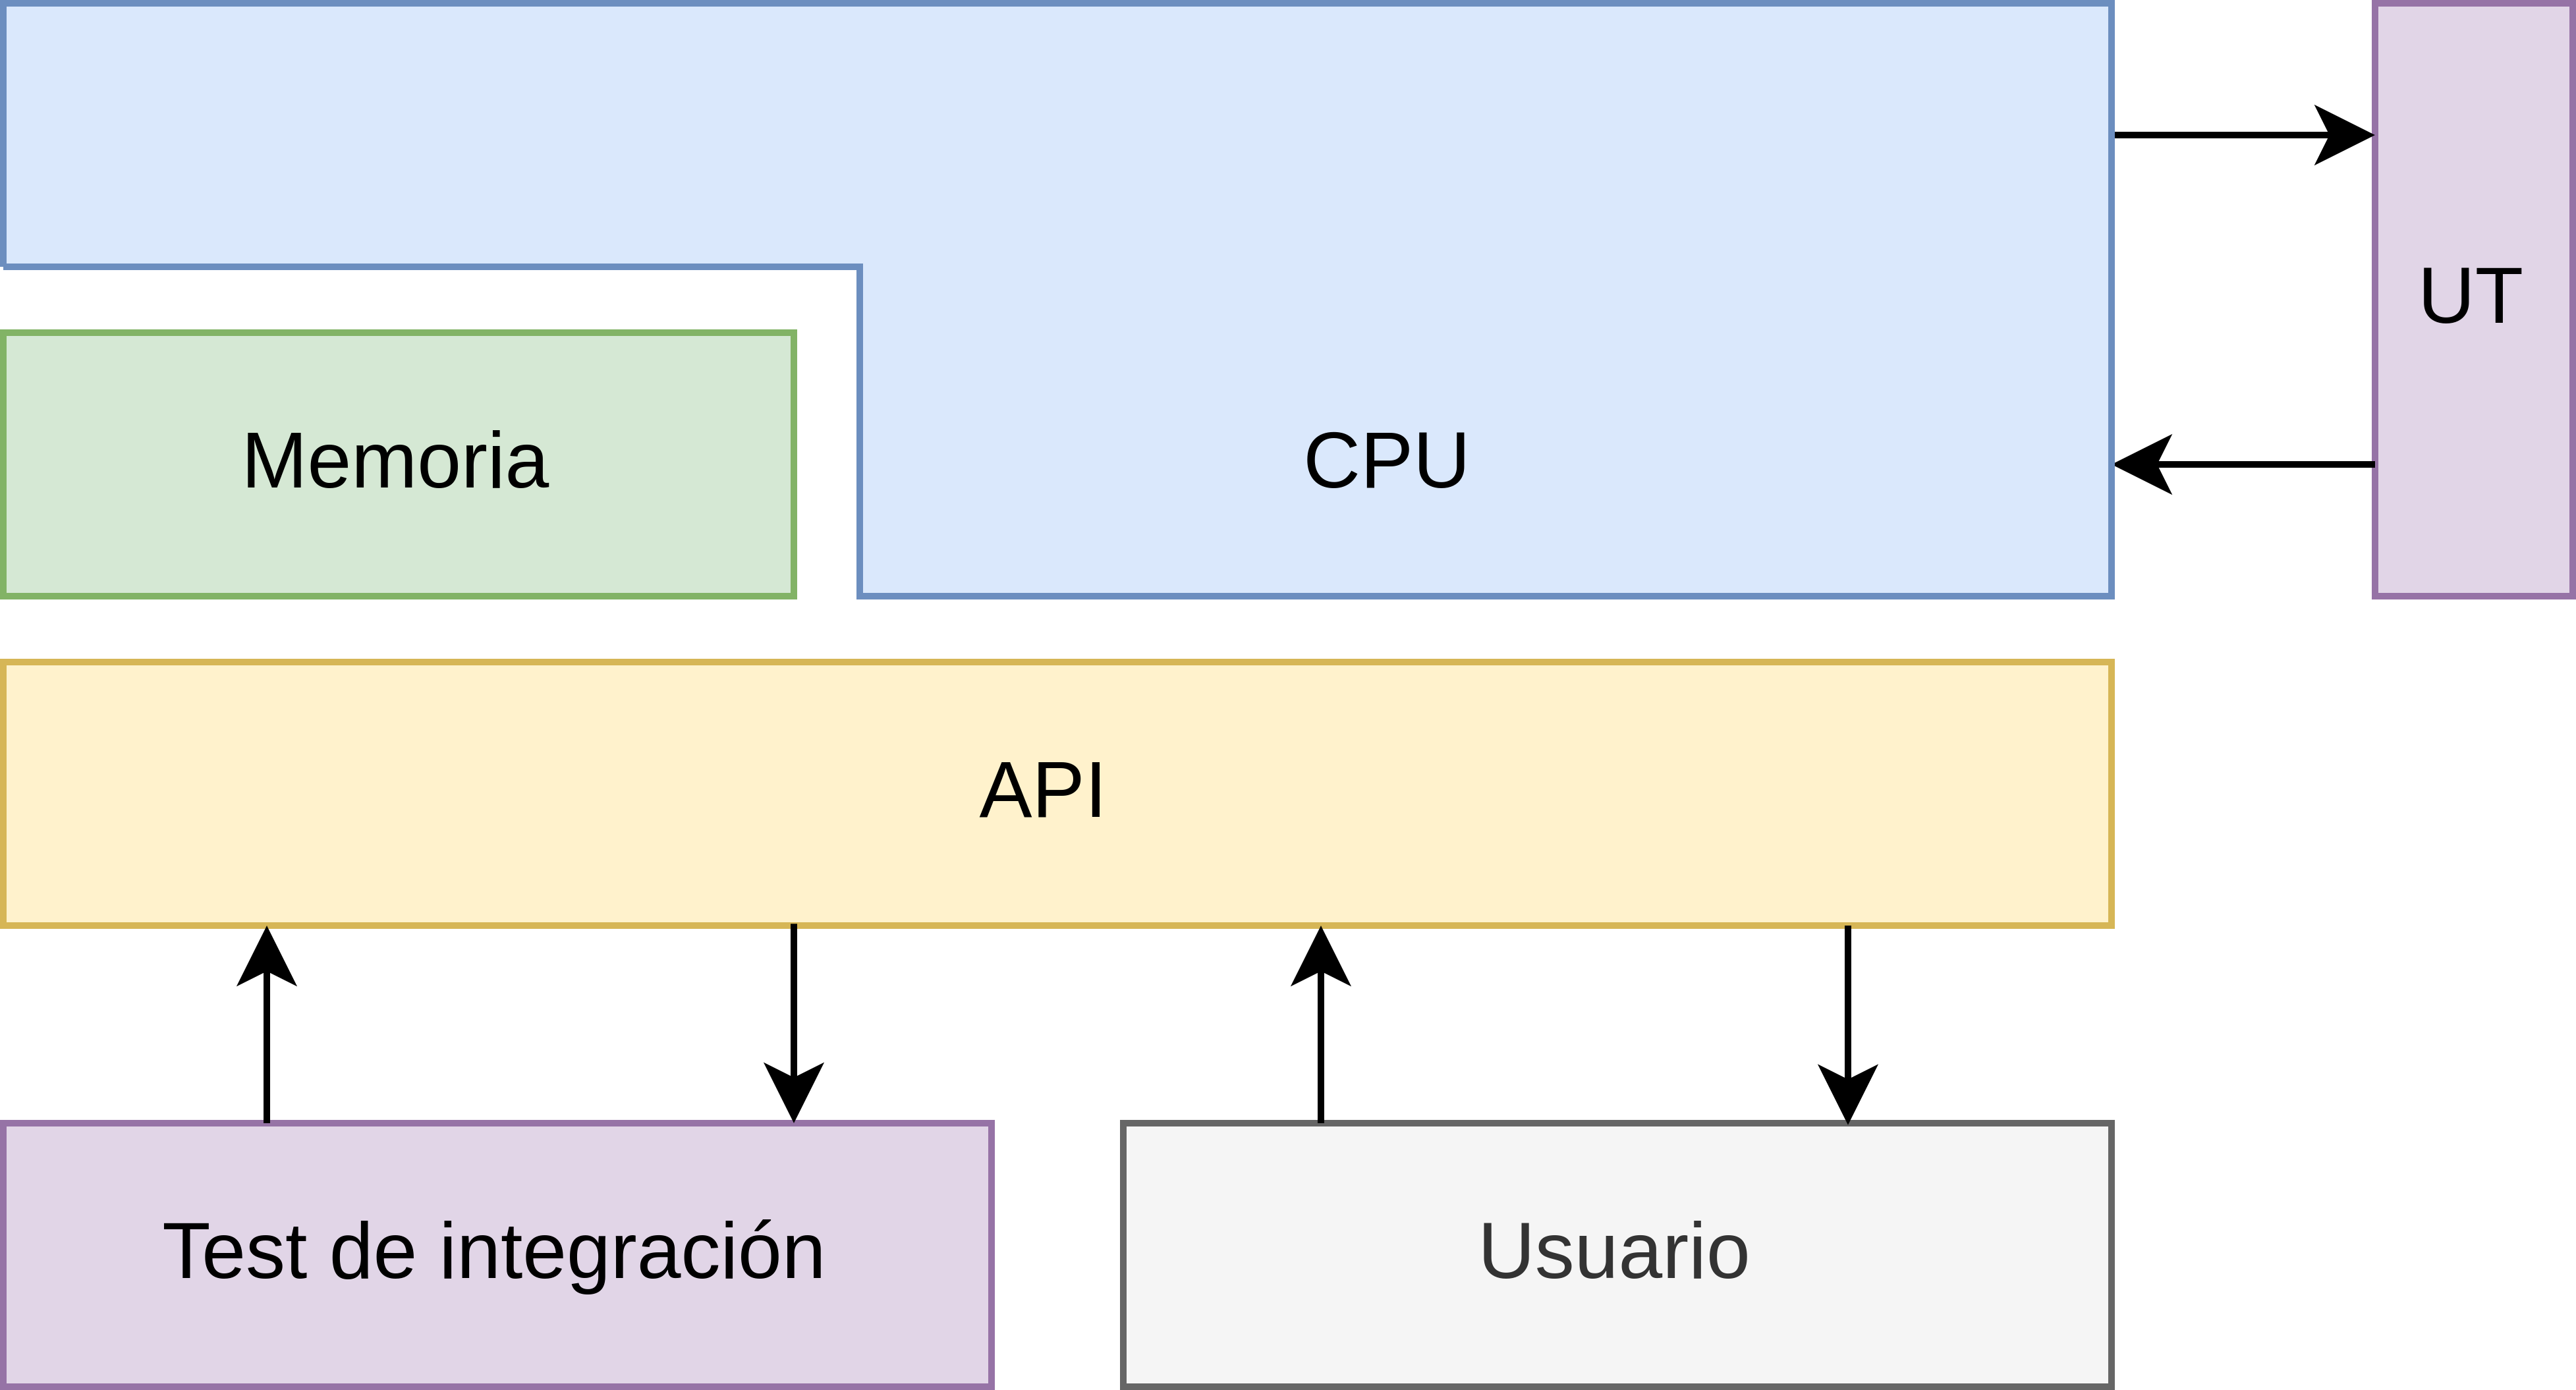
\includegraphics[width=.85\textwidth]{./Figures/diagrama_bloques}
	\caption{Diagrama en bloques del proyecto.}
	\label{fig:diagrama_bloques}
\end{figure}

Dichos componentes serán desarrollados en el transcurso del capítulo.

\begin{enumerate}
\item Memoria.
\item CPU.
\item API.
\item Tests unitarios (UT) y de integración.
\end{enumerate}

\subsection{Memoria}
\label{subsec:memoria}

En el trabajo se ha desarrollado un único modelo de memoria volátil (RAM) que consiste en un array de 32 gigabytes de tamaño. A dicho abstracción se le agregaron las operaciones de lectura y escritura de 32 bits. Por facilidad de testeo se decidió inicializar toda la memoria con ceros para discernir entre escrituras erróneas y lecturas de direcciones no inicializadas.

Una decisión técnica que se tomó con la memoria del sistema fue la de utilizar \textit{little-endian} en vez de \textit{big-endian} como lo haría el hardware real. La razón de esta decisión fue que la arquitectura x86, en la que se desarrolló el emulador, utiliza \textit{little-endian}, por lo que se evita tener que realizar conversiones de endianess en cada lectura o escritura de memoria, y dichas transformaciones fueron reubicadas en la capa de API para garantizar que el usuario final pueda observar la memoria memoria emulada con el mismo ordenamiento que en el hardware real.

Esta consideración implica que el firmware que se cargue se desee ejecutar deberá ser transformado a \textit{little-endian} durante la carga para cumplir con el requerimiento de poder ejecutar los mismos binarios que se utilizan en el hardware real.

\subsection{CPU}
\label{subsec:cpu}

\subsection{API}
\label{subsec:api}

\subsection{Tests unitarios y de integración}
\label{subsec:tests_unitarios_integracion}

----------------------------------------------------------------------------------------------------------

\textbf{NOTA:} Hasta aquí llegué, lo siguiente son borradores que se utilizarán cuando sean necesarios. Recordar de revisar el apéndice \ref{AppendixA}.

----------------------------------------------------------------------------------------------------------

%% - Breve descripcion de Firmwares y Bootloaders (software de vuelo)
%% - Descripcion de computadora a bordo
%% - Descripcion componentes a emular (Memoria RAM y microprocesador)

En el presente trabajo, no se ha modelado una memoria persistente, por lo que se ha agregado una función que recibe un archivo binario (FSW) y lo carga en la memoria RAM del sistema. Dicha funcion posicionará al binario en la dirección correcta de memoria, donde el CPU lo pueda ejecutar.

La figura \ref{fig:carga_binario} muestra un diagrama de flujo del procedimiento de carga y ejecución de un software en el emulador desarrollado. El diagrama asume que ya se posee un archivo binario valido para la arquitectura SPARC V8.

\begin{figure}[htbp]
	\centering
	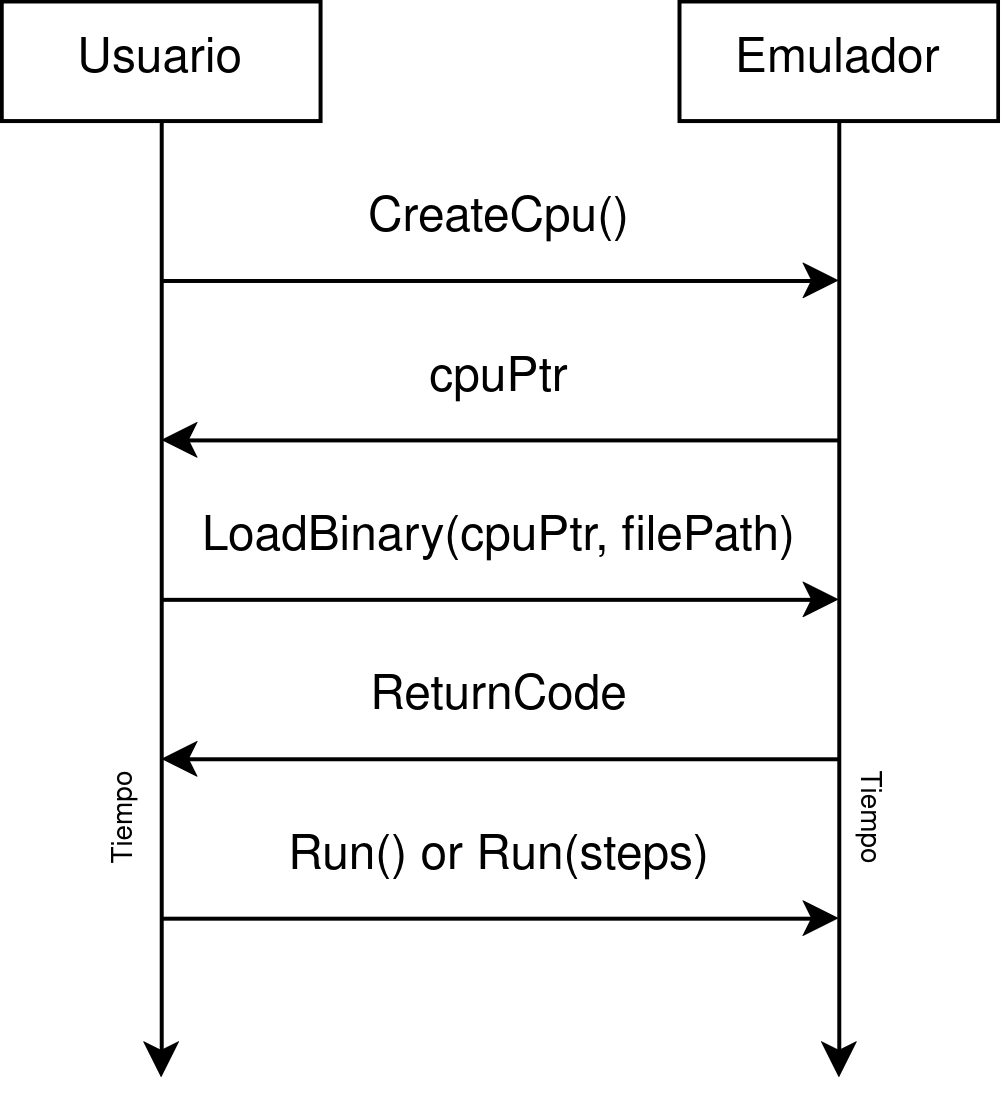
\includegraphics[width=.6\textwidth]{./Figures/carga_binario}
	\caption{Proceso de carga de binarios en emulador.}
	\label{fig:carga_binario}
\end{figure}

\newpage

Todo el procedimiento descrito anteriormente se lleva a cabo en la computadora a bordo (OBC) del sistema. La OBC es el componente que se encarga de orquestar el resto de los subsistemas del sistema. En un escenario real, la OBC tendría más componentes que los que se han modelado en este trabajo, tales como periféricos de comunicación UART, CAN y SpaceWire, entre otros. La figura \ref{fig:componentes_desarrollados}, tomada de la página de Gaisler \citep{GR712RC} y editada, muestra en detalle todos los componentes de la OBC GR712RC resaltando en rojo los componentes que se han modelado en el presente trabajo.


\begin{figure}[htbp]
	\centering
	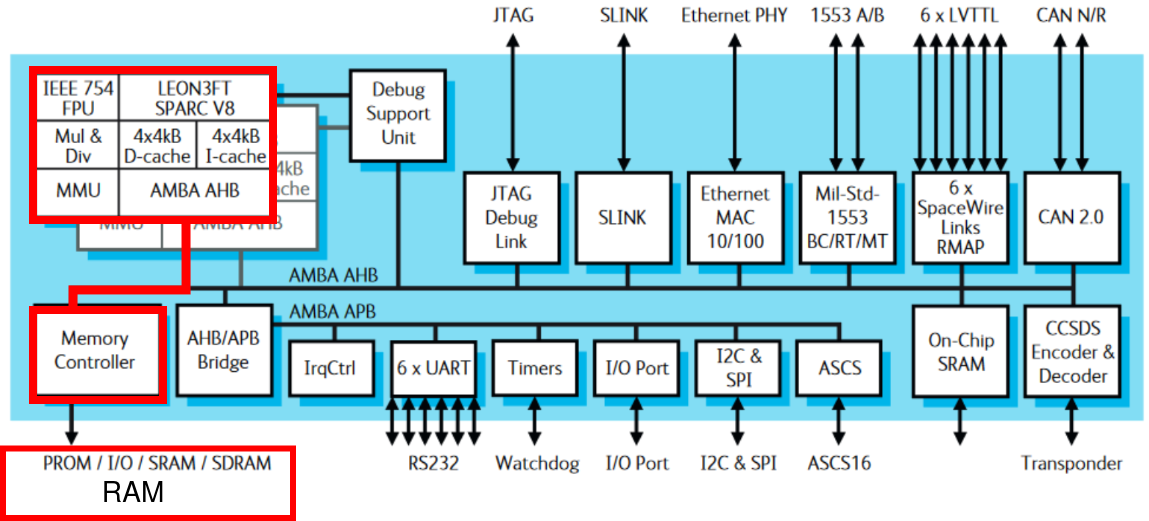
\includegraphics[width=1\textwidth]{./Figures/componentes_desarrollados}
	\caption{Componentes emulados.}
	\label{fig:componentes_desarrollados}
\end{figure}
\newpage

Cabe destacar que se utilizó la placa de desarrollo GR712RC como referencia para el desarrollo del emulador, ya que es una placa de desarrollo de uso común en aplicaciones espaciales. Se pueden destacar las siguientes simplificaciones realizadas:

\begin{itemize}
\item Se ha modelado únicamente un CPU. Esta simplificación permite omitir todas las instrucciones de sincronización y manejo de interrupciones que se deberían implementar en un sistema multi-core.
\item Se ha modelado el controlador de memoria (MCU por sus siglas en inglés \textit{Memory Controller Unit}) correctamente.
\item Las memorias PROM, I/O, SRAM y SDRAM se han modelado como un único bloque de memoria RAM. Dicha simplificación reduce significativamente el número de modelos a implementar y no afecta el funcionamiento del emulador.
\end{itemize}


Para la CPU, se desarrollaron las siguientes instrucciones de la arquitectura SPARC V8:

\begin{enumerate}

\item \texttt{UNIMP}: Genera un interrupción de procesador.
\item \texttt{Bicc}: Salto condicional (Números enteros).
\item \texttt{SETHi}: Escritura de los 22bits mas significativos de un registro.
\item \texttt{FBfcc}: Salto condicional (Números punto flotante).
\item \texttt{CBfcc}: Salto condicional (Códigos de condición).

\item \texttt{CALL}: Llamada a subrutina.

\item \texttt{ADD}: Adición.
\item \texttt{ADDcc}: Adición con código de condición.
\item \texttt{ADDX}: Adición con retorno de carro.

\item \texttt{SUB}: Sustracción.
\item \texttt{SUBcc}: Sustracción con código de condición.
\item \texttt{SUBX}: Sustracción con retorno de carro.

\item \texttt{AND}: Operación \texttt{AND} lógica.
\item \texttt{ANDcc}: Operación \texttt{AND} lógica con actualización de código de condición.
\item \texttt{ANDN}: Operación de \texttt{AND} negada lógica.

\item \texttt{OR}: Operación \texttt{OR} lógica.
\item \texttt{XOR}: Operación de \textit{exclusive or}.
\item \texttt{ORcc}: Operación \texttt{OR} lógica con actualización de código de condición.

\item \texttt{SLL}: Desplazamiento lógico a la izquierda.
\item \texttt{SRL}: Desplazamiento lógico a la derecha.
\item \texttt{SRA}: Desplazamiento aritmético a la derecha.

\item \texttt{RDPSR}: Lectura del registro de estado del procesador.

\item \texttt{RDY\_RDASR}: Lectura del registro \texttt{Y} del procesador.

\item \texttt{WRY}: Escritura del registro \texttt{Y} del procesador.
\item \texttt{WRPSR}: Escritura del registro \texttt{PSR} del procesador.
\item \texttt{WRWIM}: Escritura del registro \texttt{WIM} del procesador.
\item \texttt{WRTBR}: Escritura del registro \texttt{TBR} del procesador.

\item \texttt{TICC}: Interrupción en código de condición de enteros.

\item \texttt{JMPL}: Salto incondicional.
\item \texttt{FLUSH}: Limpieza de operaciones pendientes.
\item \texttt{SAVE}: Guardado de ventana de procesamiento.
\item \texttt{RESTORE}: Carga de ventana de procesamiento.

\end{enumerate}


\section{Consideraciones y decisiones tecnicas}
\label{sec:consideraciones_decisiones_tecnicas}

Un desafío que se tuvo que resolver temprana en el desarrollo del emulador fue la endianess del sistema. El endianess es el orden en el que se almacenan los bytes en la memoria. En el caso de la arquitectura SPARC V8, se utiliza el ordenamiento \textit{big-endian}, lo que significa que el byte más significativo se almacena en la dirección de memoria más alta. Por otro lado, la arquitectura x86 (Es decir, nuestros computadoras de escritorio) utiliza el ordenamiento \textit{little-endian}, donde el byte menos significativo se almacena en la dirección de memoria más baja. Por lo tanto, al momento de interpretar los datos obtenidos de la memoria, se debe reordenar los bytes para que tengan sentido. Dicha problemática es propia únicamente del emulado

\section{Diagrama de bloques}
\label{sec:diag_bloques}

\section{Arquitectura del software}
\label{sec:arquitectura_software}

\section{Modulos componentes del software}
\label{sec:modulos_componentes_software}


\section{Desarrollo del software}
\label{sec:desarrollo_software}


	% Chapter Template

\chapter{Ensayos y resultados} % Main chapter title

\label{Chapter4} % Change X to a consecutive number; for referencing this chapter elsewhere, use \ref{ChapterX}

%----------------------------------------------------------------------------------------
%	SECTION 1
%----------------------------------------------------------------------------------------

\section{Pruebas funcionales del hardware}
\label{sec:pruebasHW}

La idea de esta sección es explicar cómo se hicieron los ensayos, qué resultados se obtuvieron y analizarlos.
 
	% Chapter Template

\chapter{Conclusiones} % Main chapter title

\label{Chapter5} % Change X to a consecutive number; for referencing this chapter elsewhere, use \ref{ChapterX}


%----------------------------------------------------------------------------------------

%----------------------------------------------------------------------------------------
%	SECTION 1
%----------------------------------------------------------------------------------------

\section{Conclusiones generales }

La idea de esta sección es resaltar cuáles son los principales aportes del trabajo realizado y cómo se podría continuar. Debe ser especialmente breve y concisa. Es buena idea usar un listado para enumerar los logros obtenidos.

Algunas preguntas que pueden servir para completar este capítulo:

\begin{itemize}
\item ¿Cuál es el grado de cumplimiento de los requerimientos?
\item ¿Cuán fielmente se puedo seguir la planificación original (cronograma incluido)?
\item ¿Se manifestó algunos de los riesgos identificados en la planificación? ¿Fue efectivo el plan de mitigación? ¿Se debió aplicar alguna otra acción no contemplada previamente?
\item Si se debieron hacer modificaciones a lo planificado ¿Cuáles fueron las causas y los efectos?
\item ¿Qué técnicas resultaron útiles para el desarrollo del proyecto y cuáles no tanto?
\end{itemize}


%----------------------------------------------------------------------------------------
%	SECTION 2
%----------------------------------------------------------------------------------------
\section{Próximos pasos}

Acá se indica cómo se podría continuar el trabajo más adelante.
 
\end{verbatim}

Los apéndices también deben escribirse en archivos .tex separados, que se deben ubicar dentro de la carpeta \emph{Appendices}. Los apéndices vienen comentados por defecto con el caracter \code{\%} y para incluirlos simplemente se debe eliminar dicho caracter.

Finalmente, se encuentra el código para incluir la bibliografía en el documento final.  Este código tampoco debe modificarse. La metodología para trabajar las referencias bibliográficas se desarrolla en la sección \ref{sec:biblio}.
%----------------------------------------------------------------------------------------

\section{Bibliografía}
\label{sec:biblio}

Las opciones de formato de la bibliografía se controlan a través del paquete de latex \option{biblatex} que se incluye en la memoria en el archivo memoria.tex.  Estas opciones determinan cómo se generan las citas bibliográficas en el cuerpo del documento y cómo se genera la bibliografía al final de la memoria.

En el preámbulo se puede encontrar el código que incluye el paquete biblatex, que no requiere ninguna modificación del usuario de la plantilla, y que contiene las siguientes opciones:

\begin{lstlisting}
\usepackage[backend=bibtex,
	natbib=true, 
	style=numeric, 
	sorting=none]
{biblatex}
\end{lstlisting}

En el archivo \file{reference.bib} se encuentran las referencias bibliográficas que se pueden citar en el documento.  Para incorporar una nueva cita al documento lo primero es agregarla en este archivo con todos los campos necesario.  Todas las entradas bibliográficas comienzan con $@$ y una palabra que define el formato de la entrada.  Para cada formato existen campos obligatorios que deben completarse. No importa el orden en que las entradas estén definidas en el archivo .bib.  Tampoco es importante el orden en que estén definidos los campos de una entrada bibliográfica. A continuación se muestran algunos ejemplos:

\begin{lstlisting}
@ARTICLE{ARTICLE:1,
    AUTHOR="John Doe",
    TITLE="Title",
    JOURNAL="Journal",
    YEAR="2017",
}
\end{lstlisting}


\begin{lstlisting}
@BOOK{BOOK:1,
    AUTHOR="John Doe",
    TITLE="The Book without Title",
    PUBLISHER="Dummy Publisher",
    YEAR="2100",
}
\end{lstlisting}


\begin{lstlisting}
@INBOOK{BOOK:2,
    AUTHOR="John Doe",
    TITLE="The Book without Title",
    PUBLISHER="Dummy Publisher",
    YEAR="2100",
    PAGES="100-200",
}
\end{lstlisting}


\begin{lstlisting}
@MISC{WEBSITE:1,
    HOWPUBLISHED = "\url{http://example.com}",
    AUTHOR = "Intel",
    TITLE = "Example Website",
    MONTH = "12",
    YEAR = "1988",
    URLDATE = {2012-11-26}
}
\end{lstlisting}

Se debe notar que los nombres \emph{ARTICLE:1}, \emph{BOOK:1}, \emph{BOOK:2} y \emph{WEBSITE:1} son nombres de fantasía que le sirve al autor del documento para identificar la entrada. En este sentido, se podrían reemplazar por cualquier otro nombre.  Tampoco es necesario poner : seguido de un número, en los ejemplos sólo se incluye como un posible estilo para identificar las entradas.

La entradas se citan en el documento con el comando: 

\begin{verbatim}
\citep{nombre_de_la_entrada}
\end{verbatim}

Y cuando se usan, se muestran así: \citep{ARTICLE:1}, \citep{BOOK:1}, \citep{BOOK:2}, \citep{WEBSITE:1}.  Notar cómo se conforma la sección Bibliografía al final del documento.

Finalmente y como se mencionó en la subsección \ref{subsec:configurando}, para actualizar las referencias bibliográficas tanto en la sección bibliografía como las citas en el cuerpo del documento, se deben ejecutar las herramientas de compilación PDFLaTeX, BibTeX, PDFLaTeX, PDFLaTeX, en ese orden.  Este procedimiento debería resolver cualquier mensaje "Citation xxxxx on page x undefined".

	\chapter{Introducción específica} % Main chapter title

El presente capítulo describe los elementos componentes del sistema, el principio de funcionamiento y los requerimientos acordados con el cliente sobre el sistema.


\label{Chapter2}

%----------------------------------------------------------------------------------------
%	SECTION 1
%----------------------------------------------------------------------------------------


\section{Elementos componentes del sistema}
\label{sec:elementos_componentes_sistema}

Para entender el funcionamiento del sistema, es necesario conocer los elementos que lo componen. La presente sección describirá tanto los elementos físicos necesarios para conocer al sistema que se busca representar, como las herramientas de software utilizadas para el desarrollo del emulador.

\subsection{Elementos físicos del sistema}
\label{subsec:elementos_fisicos}

La presente sección dará una descripción general de los elementos que serán de vital importancia para el proyecto.

\subsubsection{Bootloader}
\label{subsec:bootloader}

El \textit{bootloader} es una pieza de software relativamente simple, cuyo principal objetivo es cargar el software de vuelo en la memoria RAM del sistema. Una vez cargado el software de vuelo, le cede el control al software de vuelo, el cual se encarga de ejecutar la misión del sistema.

En misiones espaciales es común que el \textit{bootloader} tenga la capacidad de verificar la integridad del software de vuelo antes de cargarlo en la memoria RAM, así mismo, de cargar diferentes versiones del software de vuelo en caso de que alguna de ellas se encuentre dañada.

\subsubsection{Firmware}
\label{subsec:firmware}

El \textit{firmware} es un software que se encuentra almacenado en la memoria no volátil del sistema, y es el encargado de inicializar los periféricos del sistema. Usualmente, este componente es desarrollado por un equipo especializado tanto en la misión para la que se está desarrollando el sistema, como en la arquitectura del microprocesador que se está utilizando. En el caso de aplicaciones espaciales, el \textit{firmware} es llamado software de vuelo o \textit{Fly Software} (FSW).

Normalmente, en la memoria no volátil del sistema se almacenan múltiples versiones del software de vuelo. Varias de ellas están presentes para servir de redundancia, en caso de que alguna de ellas se encuentre dañada, como para almacenar distintas versiones del software de vuelo con modos de operación más limitados pero seguros.

\subsubsection{Unidad de procesamiento}
\label{subsec:unidad_procesamiento}
Todo lo previamente mencionado se ejecuta en la unidad de procesamiento o CPU. La CPU es el componente encargado de ejecutar las instrucciones tanto del \textit{bootloader} como del software de vuelo.

El CPU interactúa con los periféricos del sistema, especialmente con la memoria RAM del sistema, ya que es el medio de almacenamiento masivo de alta velocidad de acceso.

El CPU, una vez encendido, empezará a leer las instrucciones de una posición dada por el fabricante y ejecutarlas secuencialmente. Es deber del desarrollador posicionar al \textit{bootloader} en esa posición de memoria.

\subsection{Software utilizado}
\label{subsec:software_utilizado}

La presente sección describirá las herramientas de software que fueron utilizadas para el desarrollo del trabajo.

\subsubsection{C++}
\label{subsec:cpp}

Dado que el emulador es un software que simula el comportamiento de un CPU, es necesario que el lenguaje de programación utilizado sea de bajo nivel, permitiendo mejores tiempos de ejecución y un mayor control sobre los recursos utilizados. Por lo tanto, se decidió utilizar C++ como lenguaje de programación para el desarrollo del emulador.

Otro motivo para su elección es que C++ es un lenguaje de programación ampliamente utilizado en la industria, por lo que facilita la comunicación con otros desarrolladores y la integración con otros sistemas.

\subsubsection{Herramientas Clang}
\label{subsec:clang_tidy}

Se utilizó Clang Tidy como herramienta de análisis estático de código. Permitiendo una mayor calidad del código y sintaxis uniforme. Así mismo se forzaron reglas para evitar malas prácticas comunes en los lenguajes de programación de bajo nivel, tales como el uso de memoria no inicializada, o aritmética de punteros.

También se utilizó Clang Format para mantener un estilo de código uniforme en todo el proyecto.

\subsubsection{Latex}
\label{subsec:latex}

Se utilizó Latex como herramienta de escritura de la documentación para el manual de usuario del proyecto. Dicha elección se tomo debido a que Latex es una herramienta ampliamente utilizada en la industria para la escritura de documentos técnicos.

El manual de usuario busca ser una guía completa y en detalle de la herramienta, no solo explicando la interfaz expuesta, sino decisiones de diseño y funcionamiento interno de la herramienta.

\subsubsection{Doxygen}
\label{subsec:doxygen}

Se utilizó Doxygen como herramienta de generación de documentación del código fuente. Con esta herramienta se generó un sitio web el cual describe la interfaz para interactuar con la herramienta (API). Dicha documentación busca ser una guía rápida para desarrolladores que estén utilizando el emulador.


\section{Principio de funcionamiento}
\label{sec:principio_funcionamiento}

El funcionamiento de un CPU, y por lo tanto de un emulador, se puede mostrar de manera simplificada de forma gráfica:

\begin{figure}[htbp]
	\centering
	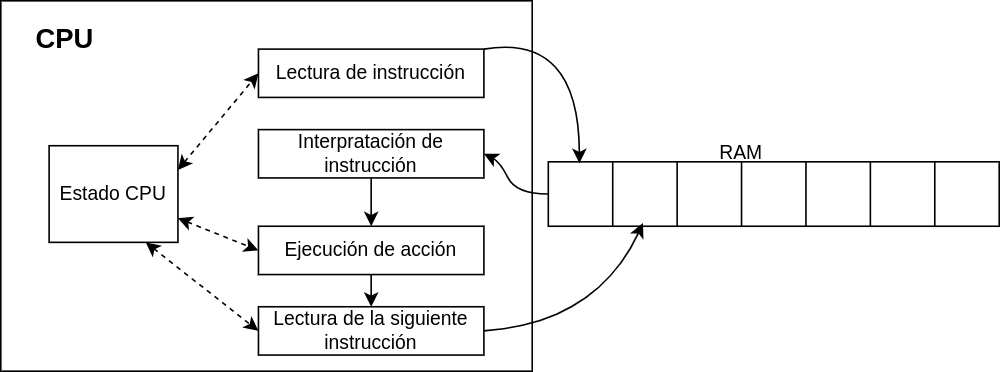
\includegraphics[width=1\textwidth]{./Figures/funcionamiento_emulador}
	\caption{Funcionamiento de alto nivel de un CPU o emulador.}
	\label{fig:functionamiento_emulador}
\end{figure}

Dicho flujo se ejecuta de manera continua, y no necesariamente las instrucciones se ejecutan en el orden en el que se encuentran en la memoria. Esto se debe a que el CPU tiene instrucciones de salto condicional, instrucciones de salto incondicional, y puede recibir interrupciones que cambien el flujo de ejecución del programa.


Un desafío que se tuvo que resolver temprana en el desarrollo del emulador fue la endianess del sistema. El endianess es el orden en el que se almacenan los bytes en la memoria. En el caso de la arquitectura SPARC V8, se utiliza el ordenamiento \textit{big-endian}, lo que significa que el byte más significativo se almacena en la dirección de memoria más alta. Por otro lado, la arquitectura x86 (Es decir, nuestros computadoras de escritorio) utiliza el ordenamiento \textit{little-endian}, donde el byte menos significativo se almacena en la dirección de memoria más baja. Por lo tanto, al momento de interpretar los datos obtenidos de la memoria, se debe reordenar los bytes para que tengan sentido. Dicha problemática es propia únicamente del emulado

\section{Requerimientos}
\label{sec:requerimientos}

 
	\chapter{Diseño e implementación} % Main chapter title
\label{Chapter3}

El presente capítulo describe los elementos componentes del sistema en detalle, las consideraciones y decisiones técnicas tomadas durante el desarrollo del emulador, el diagrama de bloques del sistema, la arquitectura del software y los módulos que lo componen.

%----------------------------------------------------------------------------------------
%	SECTION 1
%----------------------------------------------------------------------------------------


\section{Consideraciones y desiciones técnicas}
\label{sec:consideraciones_decisiones_tecnicas}

El trabajo realizado se puede dividir en cuatro grandes componentes, tal como se muestra en la figura \ref{fig:diagrama_bloques}:

\begin{figure}[htbp]
	\centering
	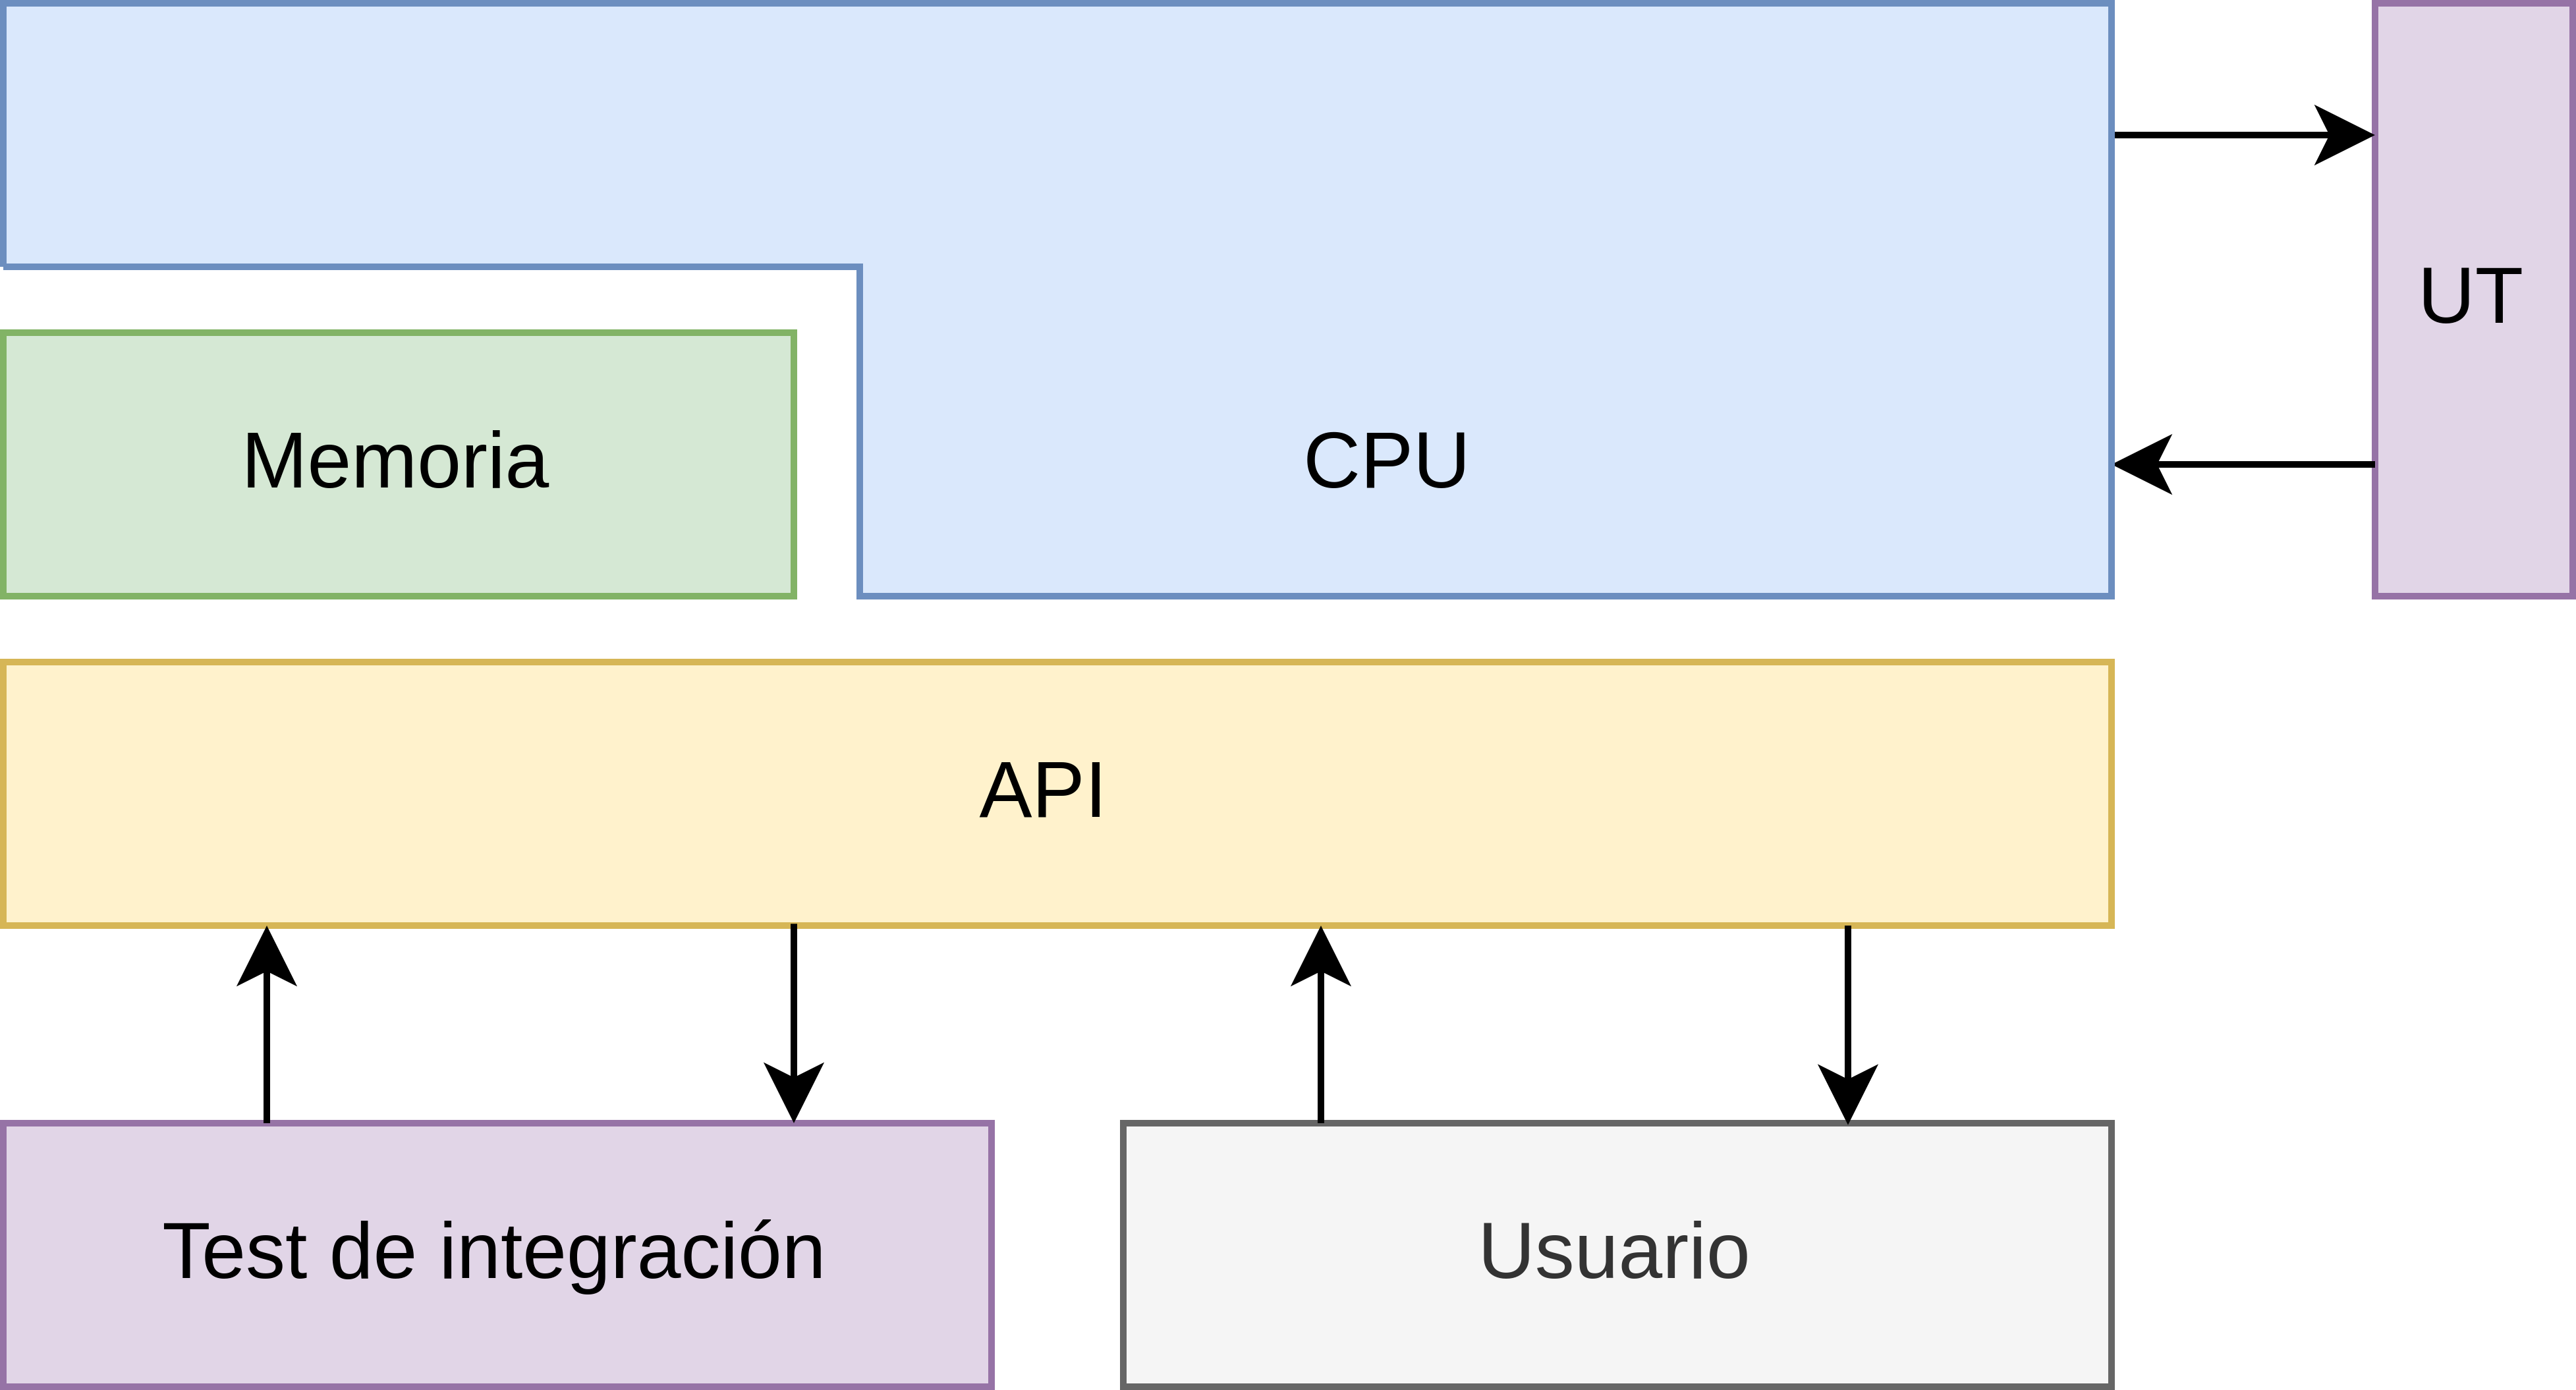
\includegraphics[width=.85\textwidth]{./Figures/diagrama_bloques}
	\caption{Diagrama en bloques del proyecto.}
	\label{fig:diagrama_bloques}
\end{figure}

Dichos componentes serán desarrollados en el transcurso del capítulo.

\begin{enumerate}
\item Memoria.
\item CPU.
\item API.
\item Tests unitarios (UT) y de integración.
\end{enumerate}

\subsection{Memoria}
\label{subsec:memoria}

En el trabajo se ha desarrollado un único modelo de memoria volátil (RAM) que consiste en un array de 32 gigabytes de tamaño. A dicho abstracción se le agregaron las operaciones de lectura y escritura de 32 bits. Por facilidad de testeo se decidió inicializar toda la memoria con ceros para discernir entre escrituras erróneas y lecturas de direcciones no inicializadas.

Una decisión técnica que se tomó con la memoria del sistema fue la de utilizar \textit{little-endian} en vez de \textit{big-endian} como lo haría el hardware real. La razón de esta decisión fue que la arquitectura x86, en la que se desarrolló el emulador, utiliza \textit{little-endian}, por lo que se evita tener que realizar conversiones de endianess en cada lectura o escritura de memoria, y dichas transformaciones fueron reubicadas en la capa de API para garantizar que el usuario final pueda observar la memoria memoria emulada con el mismo ordenamiento que en el hardware real.

Esta consideración implica que el firmware que se cargue se desee ejecutar deberá ser transformado a \textit{little-endian} durante la carga para cumplir con el requerimiento de poder ejecutar los mismos binarios que se utilizan en el hardware real.

\subsection{CPU}
\label{subsec:cpu}

\subsection{API}
\label{subsec:api}

\subsection{Tests unitarios y de integración}
\label{subsec:tests_unitarios_integracion}

----------------------------------------------------------------------------------------------------------

\textbf{NOTA:} Hasta aquí llegué, lo siguiente son borradores que se utilizarán cuando sean necesarios. Recordar de revisar el apéndice \ref{AppendixA}.

----------------------------------------------------------------------------------------------------------

%% - Breve descripcion de Firmwares y Bootloaders (software de vuelo)
%% - Descripcion de computadora a bordo
%% - Descripcion componentes a emular (Memoria RAM y microprocesador)

En el presente trabajo, no se ha modelado una memoria persistente, por lo que se ha agregado una función que recibe un archivo binario (FSW) y lo carga en la memoria RAM del sistema. Dicha funcion posicionará al binario en la dirección correcta de memoria, donde el CPU lo pueda ejecutar.

La figura \ref{fig:carga_binario} muestra un diagrama de flujo del procedimiento de carga y ejecución de un software en el emulador desarrollado. El diagrama asume que ya se posee un archivo binario valido para la arquitectura SPARC V8.

\begin{figure}[htbp]
	\centering
	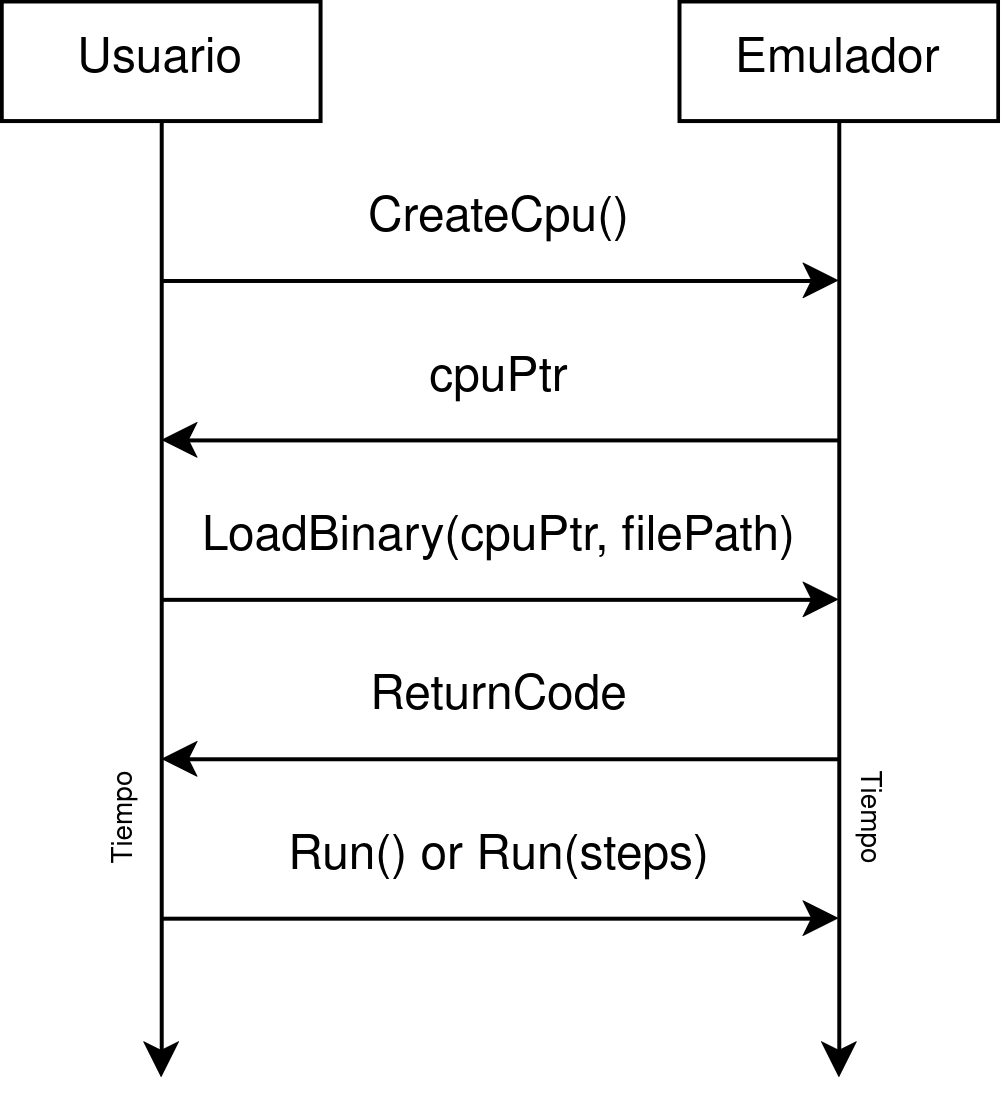
\includegraphics[width=.6\textwidth]{./Figures/carga_binario}
	\caption{Proceso de carga de binarios en emulador.}
	\label{fig:carga_binario}
\end{figure}

\newpage

Todo el procedimiento descrito anteriormente se lleva a cabo en la computadora a bordo (OBC) del sistema. La OBC es el componente que se encarga de orquestar el resto de los subsistemas del sistema. En un escenario real, la OBC tendría más componentes que los que se han modelado en este trabajo, tales como periféricos de comunicación UART, CAN y SpaceWire, entre otros. La figura \ref{fig:componentes_desarrollados}, tomada de la página de Gaisler \citep{GR712RC} y editada, muestra en detalle todos los componentes de la OBC GR712RC resaltando en rojo los componentes que se han modelado en el presente trabajo.


\begin{figure}[htbp]
	\centering
	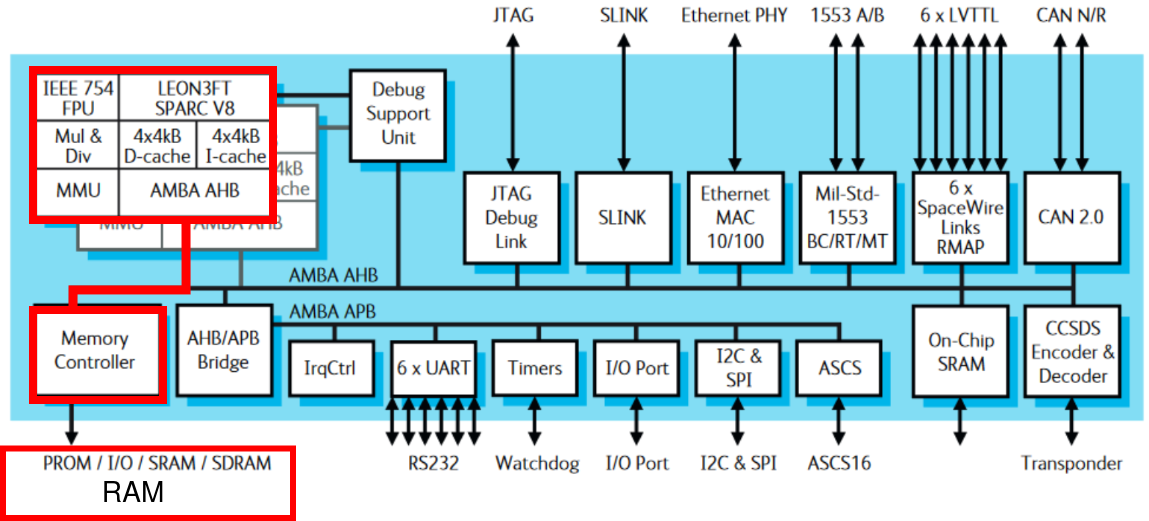
\includegraphics[width=1\textwidth]{./Figures/componentes_desarrollados}
	\caption{Componentes emulados.}
	\label{fig:componentes_desarrollados}
\end{figure}
\newpage

Cabe destacar que se utilizó la placa de desarrollo GR712RC como referencia para el desarrollo del emulador, ya que es una placa de desarrollo de uso común en aplicaciones espaciales. Se pueden destacar las siguientes simplificaciones realizadas:

\begin{itemize}
\item Se ha modelado únicamente un CPU. Esta simplificación permite omitir todas las instrucciones de sincronización y manejo de interrupciones que se deberían implementar en un sistema multi-core.
\item Se ha modelado el controlador de memoria (MCU por sus siglas en inglés \textit{Memory Controller Unit}) correctamente.
\item Las memorias PROM, I/O, SRAM y SDRAM se han modelado como un único bloque de memoria RAM. Dicha simplificación reduce significativamente el número de modelos a implementar y no afecta el funcionamiento del emulador.
\end{itemize}


Para la CPU, se desarrollaron las siguientes instrucciones de la arquitectura SPARC V8:

\begin{enumerate}

\item \texttt{UNIMP}: Genera un interrupción de procesador.
\item \texttt{Bicc}: Salto condicional (Números enteros).
\item \texttt{SETHi}: Escritura de los 22bits mas significativos de un registro.
\item \texttt{FBfcc}: Salto condicional (Números punto flotante).
\item \texttt{CBfcc}: Salto condicional (Códigos de condición).

\item \texttt{CALL}: Llamada a subrutina.

\item \texttt{ADD}: Adición.
\item \texttt{ADDcc}: Adición con código de condición.
\item \texttt{ADDX}: Adición con retorno de carro.

\item \texttt{SUB}: Sustracción.
\item \texttt{SUBcc}: Sustracción con código de condición.
\item \texttt{SUBX}: Sustracción con retorno de carro.

\item \texttt{AND}: Operación \texttt{AND} lógica.
\item \texttt{ANDcc}: Operación \texttt{AND} lógica con actualización de código de condición.
\item \texttt{ANDN}: Operación de \texttt{AND} negada lógica.

\item \texttt{OR}: Operación \texttt{OR} lógica.
\item \texttt{XOR}: Operación de \textit{exclusive or}.
\item \texttt{ORcc}: Operación \texttt{OR} lógica con actualización de código de condición.

\item \texttt{SLL}: Desplazamiento lógico a la izquierda.
\item \texttt{SRL}: Desplazamiento lógico a la derecha.
\item \texttt{SRA}: Desplazamiento aritmético a la derecha.

\item \texttt{RDPSR}: Lectura del registro de estado del procesador.

\item \texttt{RDY\_RDASR}: Lectura del registro \texttt{Y} del procesador.

\item \texttt{WRY}: Escritura del registro \texttt{Y} del procesador.
\item \texttt{WRPSR}: Escritura del registro \texttt{PSR} del procesador.
\item \texttt{WRWIM}: Escritura del registro \texttt{WIM} del procesador.
\item \texttt{WRTBR}: Escritura del registro \texttt{TBR} del procesador.

\item \texttt{TICC}: Interrupción en código de condición de enteros.

\item \texttt{JMPL}: Salto incondicional.
\item \texttt{FLUSH}: Limpieza de operaciones pendientes.
\item \texttt{SAVE}: Guardado de ventana de procesamiento.
\item \texttt{RESTORE}: Carga de ventana de procesamiento.

\end{enumerate}


\section{Consideraciones y decisiones tecnicas}
\label{sec:consideraciones_decisiones_tecnicas}

Un desafío que se tuvo que resolver temprana en el desarrollo del emulador fue la endianess del sistema. El endianess es el orden en el que se almacenan los bytes en la memoria. En el caso de la arquitectura SPARC V8, se utiliza el ordenamiento \textit{big-endian}, lo que significa que el byte más significativo se almacena en la dirección de memoria más alta. Por otro lado, la arquitectura x86 (Es decir, nuestros computadoras de escritorio) utiliza el ordenamiento \textit{little-endian}, donde el byte menos significativo se almacena en la dirección de memoria más baja. Por lo tanto, al momento de interpretar los datos obtenidos de la memoria, se debe reordenar los bytes para que tengan sentido. Dicha problemática es propia únicamente del emulado

\section{Diagrama de bloques}
\label{sec:diag_bloques}

\section{Arquitectura del software}
\label{sec:arquitectura_software}

\section{Modulos componentes del software}
\label{sec:modulos_componentes_software}


\section{Desarrollo del software}
\label{sec:desarrollo_software}


	% Chapter Template

\chapter{Ensayos y resultados} % Main chapter title

\label{Chapter4} % Change X to a consecutive number; for referencing this chapter elsewhere, use \ref{ChapterX}

%----------------------------------------------------------------------------------------
%	SECTION 1
%----------------------------------------------------------------------------------------

\section{Pruebas funcionales del hardware}
\label{sec:pruebasHW}

La idea de esta sección es explicar cómo se hicieron los ensayos, qué resultados se obtuvieron y analizarlos.
 
	% Chapter Template

\chapter{Conclusiones} % Main chapter title

\label{Chapter5} % Change X to a consecutive number; for referencing this chapter elsewhere, use \ref{ChapterX}


%----------------------------------------------------------------------------------------

%----------------------------------------------------------------------------------------
%	SECTION 1
%----------------------------------------------------------------------------------------

\section{Conclusiones generales }

La idea de esta sección es resaltar cuáles son los principales aportes del trabajo realizado y cómo se podría continuar. Debe ser especialmente breve y concisa. Es buena idea usar un listado para enumerar los logros obtenidos.

Algunas preguntas que pueden servir para completar este capítulo:

\begin{itemize}
\item ¿Cuál es el grado de cumplimiento de los requerimientos?
\item ¿Cuán fielmente se puedo seguir la planificación original (cronograma incluido)?
\item ¿Se manifestó algunos de los riesgos identificados en la planificación? ¿Fue efectivo el plan de mitigación? ¿Se debió aplicar alguna otra acción no contemplada previamente?
\item Si se debieron hacer modificaciones a lo planificado ¿Cuáles fueron las causas y los efectos?
\item ¿Qué técnicas resultaron útiles para el desarrollo del proyecto y cuáles no tanto?
\end{itemize}


%----------------------------------------------------------------------------------------
%	SECTION 2
%----------------------------------------------------------------------------------------
\section{Próximos pasos}

Acá se indica cómo se podría continuar el trabajo más adelante.
 
\end{verbatim}

Los apéndices también deben escribirse en archivos .tex separados, que se deben ubicar dentro de la carpeta \emph{Appendices}. Los apéndices vienen comentados por defecto con el caracter \code{\%} y para incluirlos simplemente se debe eliminar dicho caracter.

Finalmente, se encuentra el código para incluir la bibliografía en el documento final.  Este código tampoco debe modificarse. La metodología para trabajar las referencias bibliográficas se desarrolla en la sección \ref{sec:biblio}.
%----------------------------------------------------------------------------------------

\section{Bibliografía}
\label{sec:biblio}

Las opciones de formato de la bibliografía se controlan a través del paquete de latex \option{biblatex} que se incluye en la memoria en el archivo memoria.tex.  Estas opciones determinan cómo se generan las citas bibliográficas en el cuerpo del documento y cómo se genera la bibliografía al final de la memoria.

En el preámbulo se puede encontrar el código que incluye el paquete biblatex, que no requiere ninguna modificación del usuario de la plantilla, y que contiene las siguientes opciones:

\begin{lstlisting}
\usepackage[backend=bibtex,
	natbib=true, 
	style=numeric, 
	sorting=none]
{biblatex}
\end{lstlisting}

En el archivo \file{reference.bib} se encuentran las referencias bibliográficas que se pueden citar en el documento.  Para incorporar una nueva cita al documento lo primero es agregarla en este archivo con todos los campos necesario.  Todas las entradas bibliográficas comienzan con $@$ y una palabra que define el formato de la entrada.  Para cada formato existen campos obligatorios que deben completarse. No importa el orden en que las entradas estén definidas en el archivo .bib.  Tampoco es importante el orden en que estén definidos los campos de una entrada bibliográfica. A continuación se muestran algunos ejemplos:

\begin{lstlisting}
@ARTICLE{ARTICLE:1,
    AUTHOR="John Doe",
    TITLE="Title",
    JOURNAL="Journal",
    YEAR="2017",
}
\end{lstlisting}


\begin{lstlisting}
@BOOK{BOOK:1,
    AUTHOR="John Doe",
    TITLE="The Book without Title",
    PUBLISHER="Dummy Publisher",
    YEAR="2100",
}
\end{lstlisting}


\begin{lstlisting}
@INBOOK{BOOK:2,
    AUTHOR="John Doe",
    TITLE="The Book without Title",
    PUBLISHER="Dummy Publisher",
    YEAR="2100",
    PAGES="100-200",
}
\end{lstlisting}


\begin{lstlisting}
@MISC{WEBSITE:1,
    HOWPUBLISHED = "\url{http://example.com}",
    AUTHOR = "Intel",
    TITLE = "Example Website",
    MONTH = "12",
    YEAR = "1988",
    URLDATE = {2012-11-26}
}
\end{lstlisting}

Se debe notar que los nombres \emph{ARTICLE:1}, \emph{BOOK:1}, \emph{BOOK:2} y \emph{WEBSITE:1} son nombres de fantasía que le sirve al autor del documento para identificar la entrada. En este sentido, se podrían reemplazar por cualquier otro nombre.  Tampoco es necesario poner : seguido de un número, en los ejemplos sólo se incluye como un posible estilo para identificar las entradas.

La entradas se citan en el documento con el comando: 

\begin{verbatim}
\citep{nombre_de_la_entrada}
\end{verbatim}

Y cuando se usan, se muestran así: \citep{ARTICLE:1}, \citep{BOOK:1}, \citep{BOOK:2}, \citep{WEBSITE:1}.  Notar cómo se conforma la sección Bibliografía al final del documento.

Finalmente y como se mencionó en la subsección \ref{subsec:configurando}, para actualizar las referencias bibliográficas tanto en la sección bibliografía como las citas en el cuerpo del documento, se deben ejecutar las herramientas de compilación PDFLaTeX, BibTeX, PDFLaTeX, PDFLaTeX, en ese orden.  Este procedimiento debería resolver cualquier mensaje "Citation xxxxx on page x undefined".

\chapter{Introducción específica} % Main chapter title

El presente capítulo describe los elementos componentes del sistema, el principio de funcionamiento y los requerimientos acordados con el cliente sobre el sistema.


\label{Chapter2}

%----------------------------------------------------------------------------------------
%	SECTION 1
%----------------------------------------------------------------------------------------


\section{Elementos componentes del sistema}
\label{sec:elementos_componentes_sistema}

Para entender el funcionamiento del sistema, es necesario conocer los elementos que lo componen. La presente sección describirá tanto los elementos físicos necesarios para conocer al sistema que se busca representar, como las herramientas de software utilizadas para el desarrollo del emulador.

\subsection{Elementos físicos del sistema}
\label{subsec:elementos_fisicos}

La presente sección dará una descripción general de los elementos que serán de vital importancia para el proyecto.

\subsubsection{Bootloader}
\label{subsec:bootloader}

El \textit{bootloader} es una pieza de software relativamente simple, cuyo principal objetivo es cargar el software de vuelo en la memoria RAM del sistema. Una vez cargado el software de vuelo, le cede el control al software de vuelo, el cual se encarga de ejecutar la misión del sistema.

En misiones espaciales es común que el \textit{bootloader} tenga la capacidad de verificar la integridad del software de vuelo antes de cargarlo en la memoria RAM, así mismo, de cargar diferentes versiones del software de vuelo en caso de que alguna de ellas se encuentre dañada.

\subsubsection{Firmware}
\label{subsec:firmware}

El \textit{firmware} es un software que se encuentra almacenado en la memoria no volátil del sistema, y es el encargado de inicializar los periféricos del sistema. Usualmente, este componente es desarrollado por un equipo especializado tanto en la misión para la que se está desarrollando el sistema, como en la arquitectura del microprocesador que se está utilizando. En el caso de aplicaciones espaciales, el \textit{firmware} es llamado software de vuelo o \textit{Fly Software} (FSW).

Normalmente, en la memoria no volátil del sistema se almacenan múltiples versiones del software de vuelo. Varias de ellas están presentes para servir de redundancia, en caso de que alguna de ellas se encuentre dañada, como para almacenar distintas versiones del software de vuelo con modos de operación más limitados pero seguros.

\subsubsection{Unidad de procesamiento}
\label{subsec:unidad_procesamiento}
Todo lo previamente mencionado se ejecuta en la unidad de procesamiento o CPU. La CPU es el componente encargado de ejecutar las instrucciones tanto del \textit{bootloader} como del software de vuelo.

El CPU interactúa con los periféricos del sistema, especialmente con la memoria RAM del sistema, ya que es el medio de almacenamiento masivo de alta velocidad de acceso.

El CPU, una vez encendido, empezará a leer las instrucciones de una posición dada por el fabricante y ejecutarlas secuencialmente. Es deber del desarrollador posicionar al \textit{bootloader} en esa posición de memoria.

\subsection{Software utilizado}
\label{subsec:software_utilizado}

La presente sección describirá las herramientas de software que fueron utilizadas para el desarrollo del trabajo.

\subsubsection{C++}
\label{subsec:cpp}

Dado que el emulador es un software que simula el comportamiento de un CPU, es necesario que el lenguaje de programación utilizado sea de bajo nivel, permitiendo mejores tiempos de ejecución y un mayor control sobre los recursos utilizados. Por lo tanto, se decidió utilizar C++ como lenguaje de programación para el desarrollo del emulador.

Otro motivo para su elección es que C++ es un lenguaje de programación ampliamente utilizado en la industria, por lo que facilita la comunicación con otros desarrolladores y la integración con otros sistemas.

\subsubsection{Herramientas Clang}
\label{subsec:clang_tidy}

Se utilizó Clang Tidy como herramienta de análisis estático de código. Permitiendo una mayor calidad del código y sintaxis uniforme. Así mismo se forzaron reglas para evitar malas prácticas comunes en los lenguajes de programación de bajo nivel, tales como el uso de memoria no inicializada, o aritmética de punteros.

También se utilizó Clang Format para mantener un estilo de código uniforme en todo el proyecto.

\subsubsection{Latex}
\label{subsec:latex}

Se utilizó Latex como herramienta de escritura de la documentación para el manual de usuario del proyecto. Dicha elección se tomo debido a que Latex es una herramienta ampliamente utilizada en la industria para la escritura de documentos técnicos.

El manual de usuario busca ser una guía completa y en detalle de la herramienta, no solo explicando la interfaz expuesta, sino decisiones de diseño y funcionamiento interno de la herramienta.

\subsubsection{Doxygen}
\label{subsec:doxygen}

Se utilizó Doxygen como herramienta de generación de documentación del código fuente. Con esta herramienta se generó un sitio web el cual describe la interfaz para interactuar con la herramienta (API). Dicha documentación busca ser una guía rápida para desarrolladores que estén utilizando el emulador.


\section{Principio de funcionamiento}
\label{sec:principio_funcionamiento}

El funcionamiento de un CPU, y por lo tanto de un emulador, se puede mostrar de manera simplificada de forma gráfica:

\begin{figure}[htbp]
	\centering
	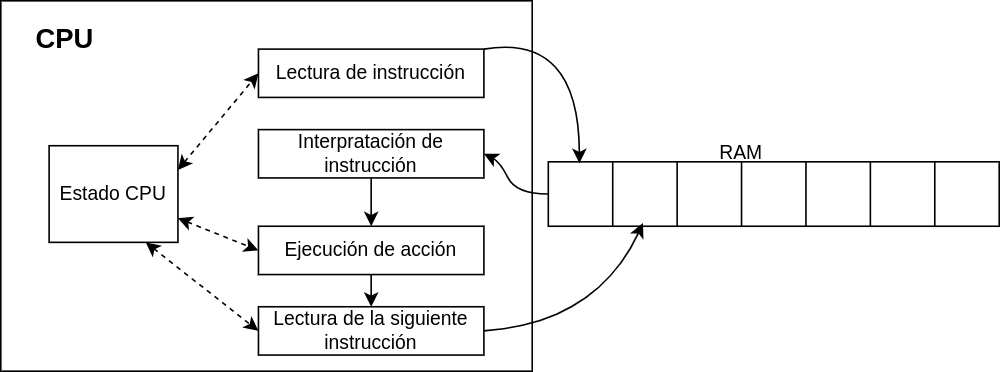
\includegraphics[width=1\textwidth]{./Figures/funcionamiento_emulador}
	\caption{Funcionamiento de alto nivel de un CPU o emulador.}
	\label{fig:functionamiento_emulador}
\end{figure}

Dicho flujo se ejecuta de manera continua, y no necesariamente las instrucciones se ejecutan en el orden en el que se encuentran en la memoria. Esto se debe a que el CPU tiene instrucciones de salto condicional, instrucciones de salto incondicional, y puede recibir interrupciones que cambien el flujo de ejecución del programa.


Un desafío que se tuvo que resolver temprana en el desarrollo del emulador fue la endianess del sistema. El endianess es el orden en el que se almacenan los bytes en la memoria. En el caso de la arquitectura SPARC V8, se utiliza el ordenamiento \textit{big-endian}, lo que significa que el byte más significativo se almacena en la dirección de memoria más alta. Por otro lado, la arquitectura x86 (Es decir, nuestros computadoras de escritorio) utiliza el ordenamiento \textit{little-endian}, donde el byte menos significativo se almacena en la dirección de memoria más baja. Por lo tanto, al momento de interpretar los datos obtenidos de la memoria, se debe reordenar los bytes para que tengan sentido. Dicha problemática es propia únicamente del emulado

\section{Requerimientos}
\label{sec:requerimientos}

 
\chapter{Diseño e implementación} % Main chapter title
\label{Chapter3}

El presente capítulo describe los elementos componentes del sistema en detalle, las consideraciones y decisiones técnicas tomadas durante el desarrollo del emulador, el diagrama de bloques del sistema, la arquitectura del software y los módulos que lo componen.

%----------------------------------------------------------------------------------------
%	SECTION 1
%----------------------------------------------------------------------------------------


\section{Consideraciones y desiciones técnicas}
\label{sec:consideraciones_decisiones_tecnicas}

El trabajo realizado se puede dividir en cuatro grandes componentes, tal como se muestra en la figura \ref{fig:diagrama_bloques}:

\begin{figure}[htbp]
	\centering
	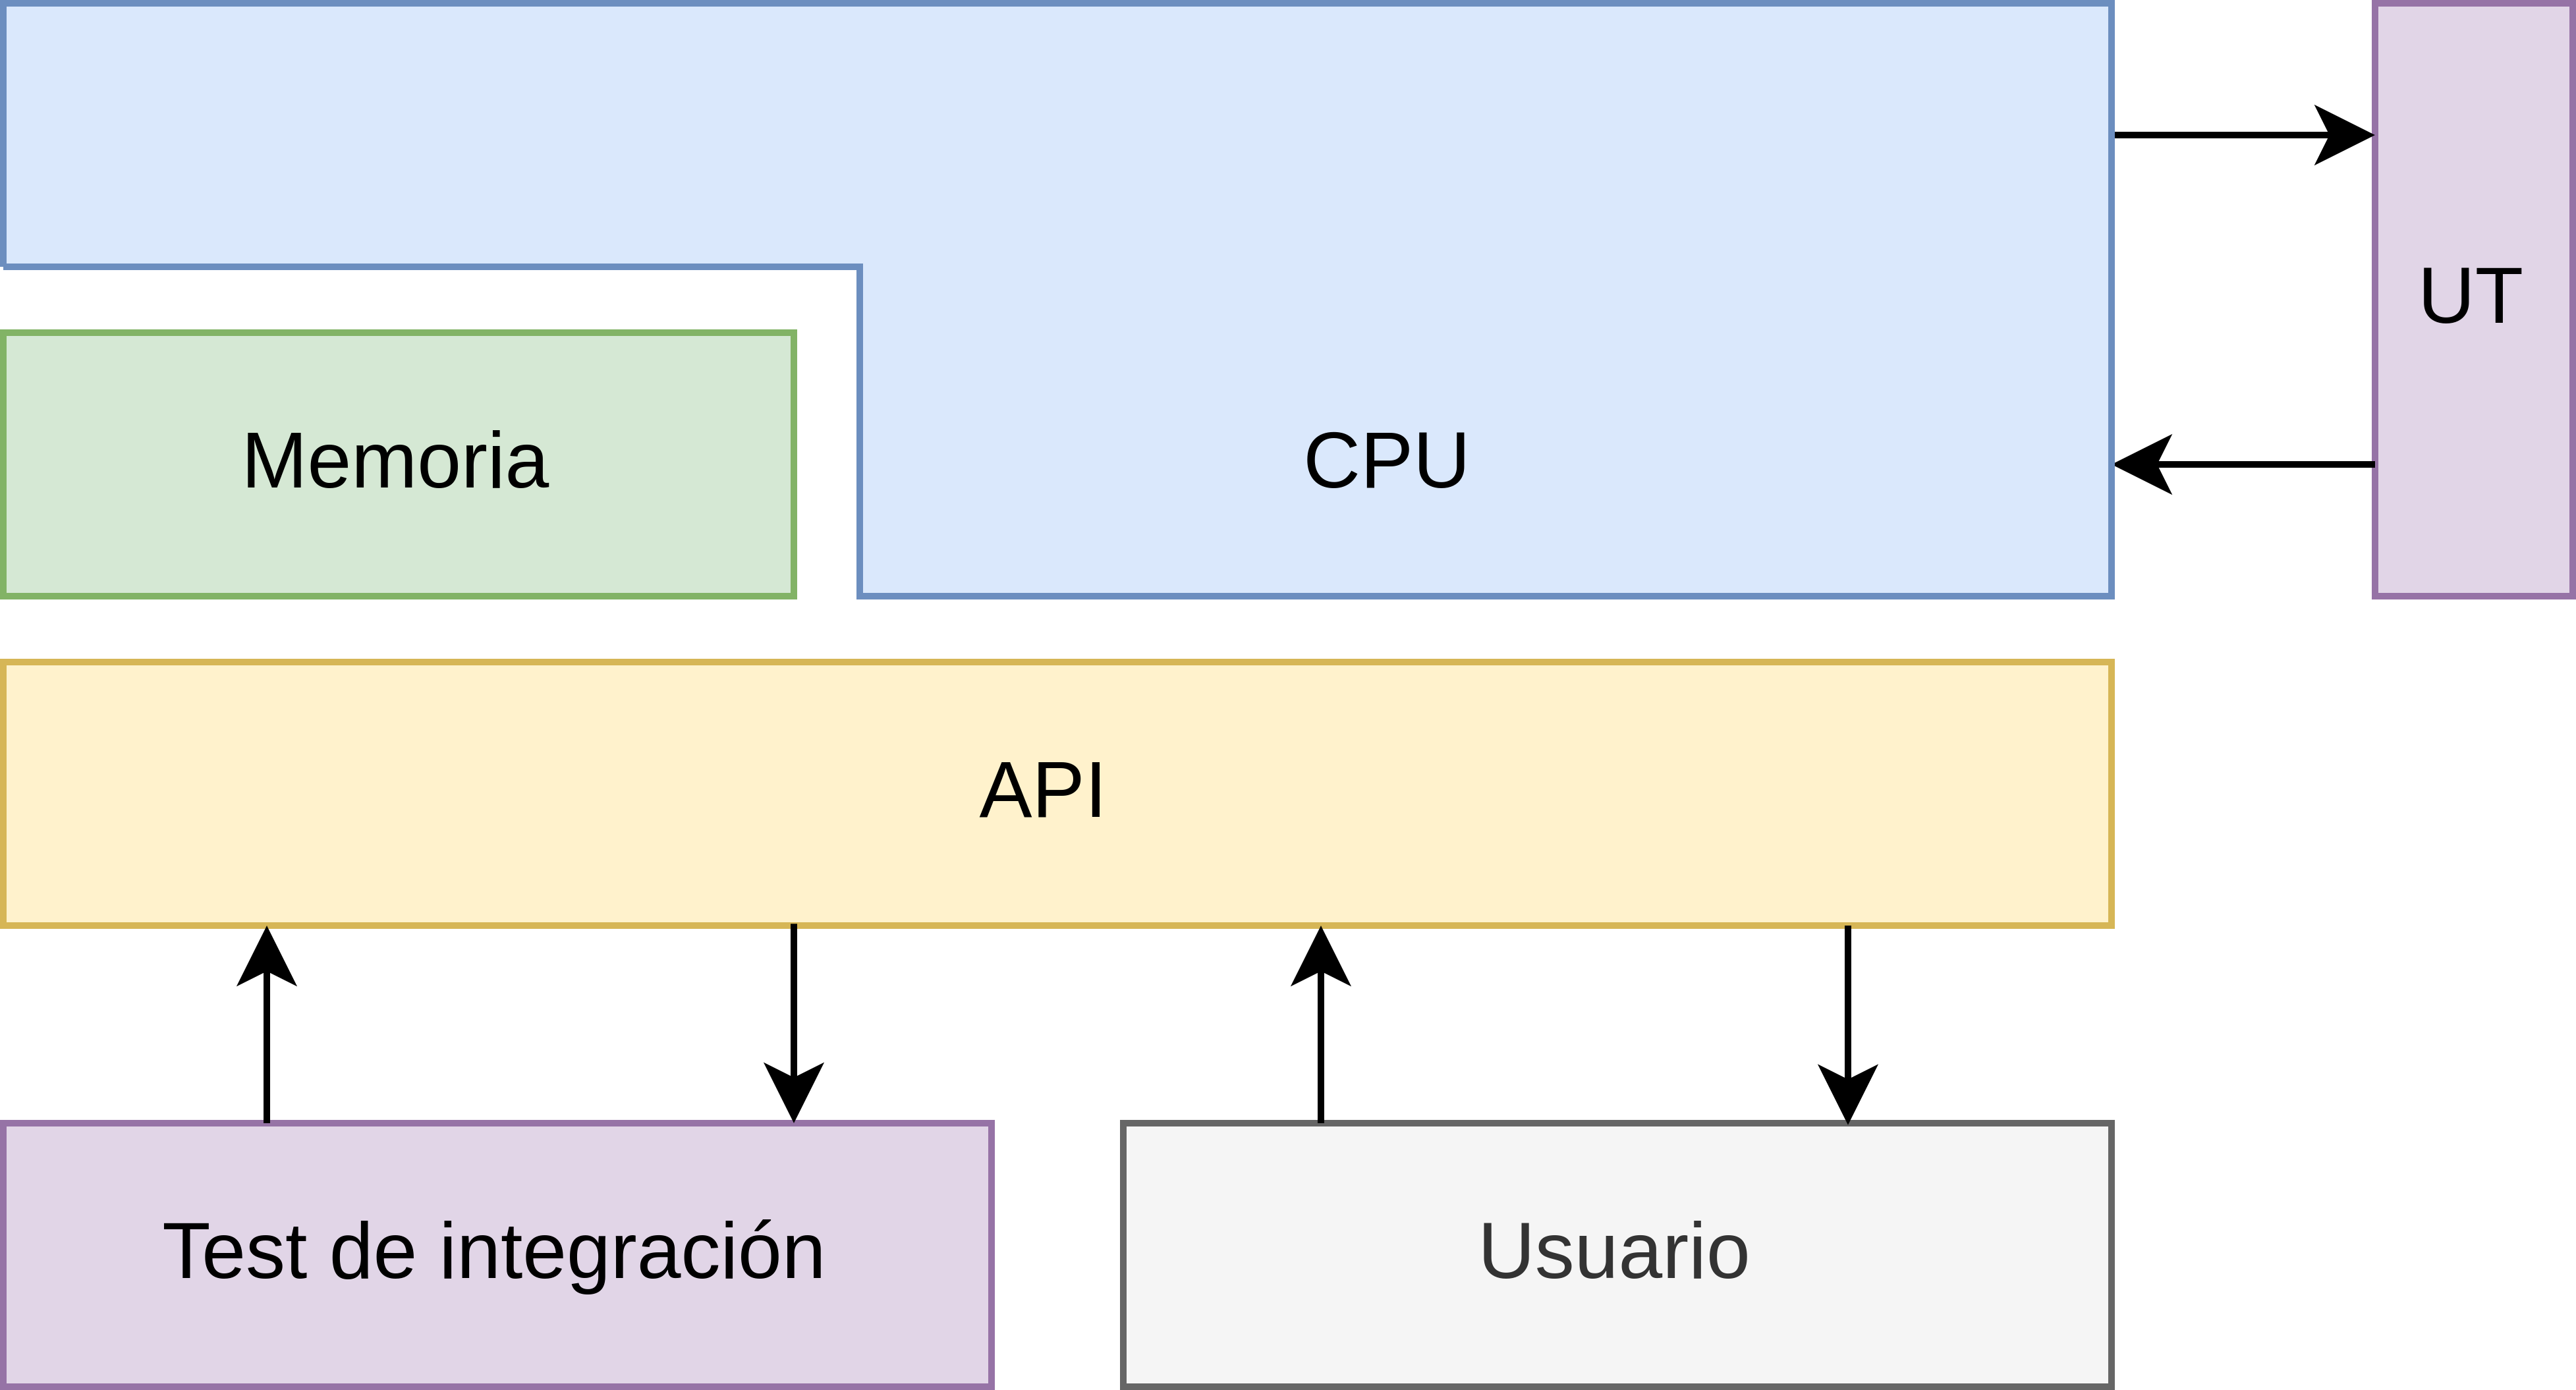
\includegraphics[width=.85\textwidth]{./Figures/diagrama_bloques}
	\caption{Diagrama en bloques del proyecto.}
	\label{fig:diagrama_bloques}
\end{figure}

Dichos componentes serán desarrollados en el transcurso del capítulo.

\begin{enumerate}
\item Memoria.
\item CPU.
\item API.
\item Tests unitarios (UT) y de integración.
\end{enumerate}

\subsection{Memoria}
\label{subsec:memoria}

En el trabajo se ha desarrollado un único modelo de memoria volátil (RAM) que consiste en un array de 32 gigabytes de tamaño. A dicho abstracción se le agregaron las operaciones de lectura y escritura de 32 bits. Por facilidad de testeo se decidió inicializar toda la memoria con ceros para discernir entre escrituras erróneas y lecturas de direcciones no inicializadas.

Una decisión técnica que se tomó con la memoria del sistema fue la de utilizar \textit{little-endian} en vez de \textit{big-endian} como lo haría el hardware real. La razón de esta decisión fue que la arquitectura x86, en la que se desarrolló el emulador, utiliza \textit{little-endian}, por lo que se evita tener que realizar conversiones de endianess en cada lectura o escritura de memoria, y dichas transformaciones fueron reubicadas en la capa de API para garantizar que el usuario final pueda observar la memoria memoria emulada con el mismo ordenamiento que en el hardware real.

Esta consideración implica que el firmware que se cargue se desee ejecutar deberá ser transformado a \textit{little-endian} durante la carga para cumplir con el requerimiento de poder ejecutar los mismos binarios que se utilizan en el hardware real.

\subsection{CPU}
\label{subsec:cpu}

\subsection{API}
\label{subsec:api}

\subsection{Tests unitarios y de integración}
\label{subsec:tests_unitarios_integracion}

----------------------------------------------------------------------------------------------------------

\textbf{NOTA:} Hasta aquí llegué, lo siguiente son borradores que se utilizarán cuando sean necesarios. Recordar de revisar el apéndice \ref{AppendixA}.

----------------------------------------------------------------------------------------------------------

%% - Breve descripcion de Firmwares y Bootloaders (software de vuelo)
%% - Descripcion de computadora a bordo
%% - Descripcion componentes a emular (Memoria RAM y microprocesador)

En el presente trabajo, no se ha modelado una memoria persistente, por lo que se ha agregado una función que recibe un archivo binario (FSW) y lo carga en la memoria RAM del sistema. Dicha funcion posicionará al binario en la dirección correcta de memoria, donde el CPU lo pueda ejecutar.

La figura \ref{fig:carga_binario} muestra un diagrama de flujo del procedimiento de carga y ejecución de un software en el emulador desarrollado. El diagrama asume que ya se posee un archivo binario valido para la arquitectura SPARC V8.

\begin{figure}[htbp]
	\centering
	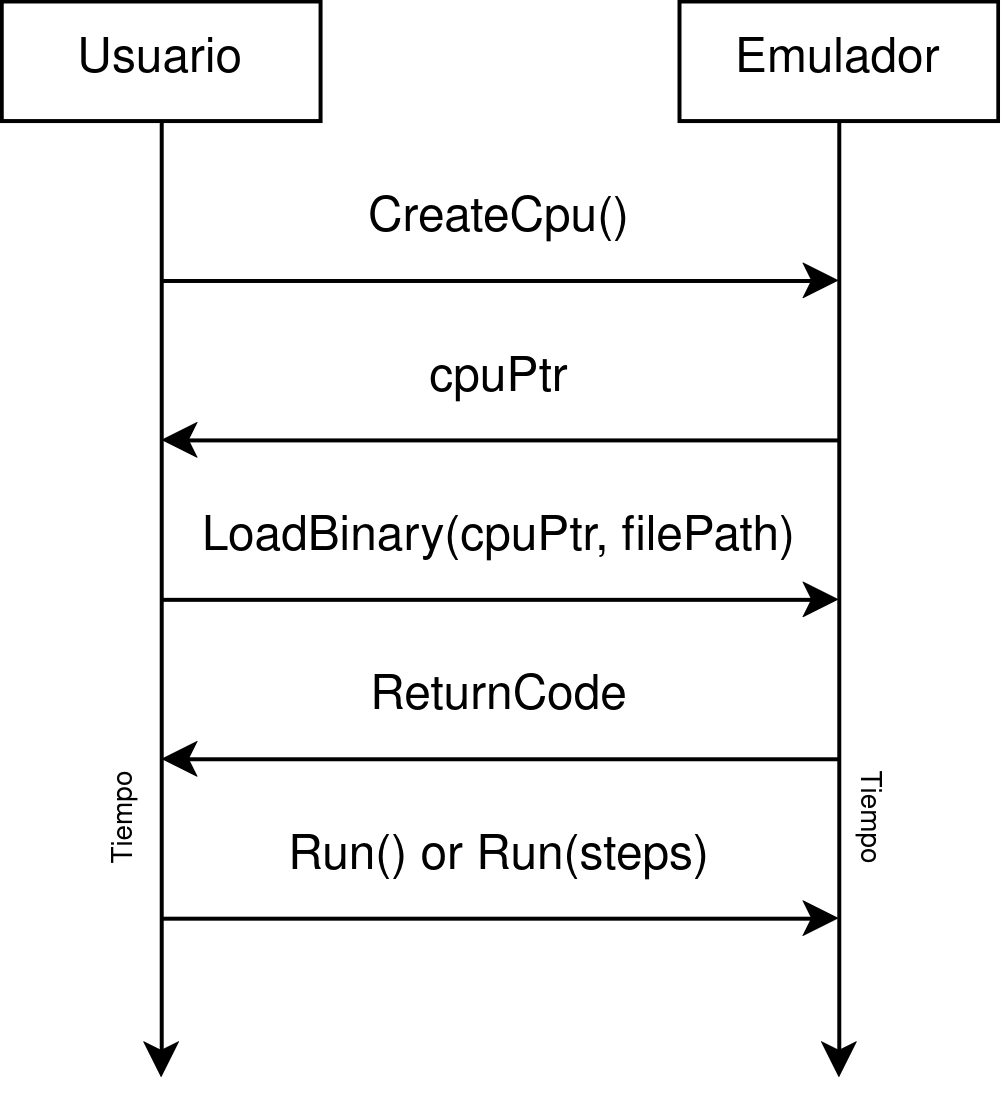
\includegraphics[width=.6\textwidth]{./Figures/carga_binario}
	\caption{Proceso de carga de binarios en emulador.}
	\label{fig:carga_binario}
\end{figure}

\newpage

Todo el procedimiento descrito anteriormente se lleva a cabo en la computadora a bordo (OBC) del sistema. La OBC es el componente que se encarga de orquestar el resto de los subsistemas del sistema. En un escenario real, la OBC tendría más componentes que los que se han modelado en este trabajo, tales como periféricos de comunicación UART, CAN y SpaceWire, entre otros. La figura \ref{fig:componentes_desarrollados}, tomada de la página de Gaisler \citep{GR712RC} y editada, muestra en detalle todos los componentes de la OBC GR712RC resaltando en rojo los componentes que se han modelado en el presente trabajo.


\begin{figure}[htbp]
	\centering
	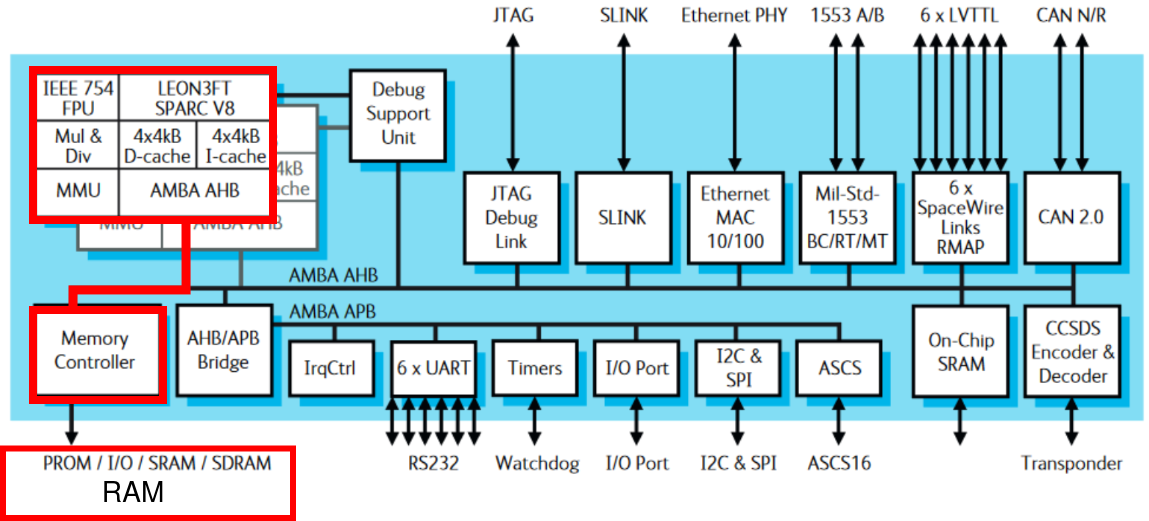
\includegraphics[width=1\textwidth]{./Figures/componentes_desarrollados}
	\caption{Componentes emulados.}
	\label{fig:componentes_desarrollados}
\end{figure}
\newpage

Cabe destacar que se utilizó la placa de desarrollo GR712RC como referencia para el desarrollo del emulador, ya que es una placa de desarrollo de uso común en aplicaciones espaciales. Se pueden destacar las siguientes simplificaciones realizadas:

\begin{itemize}
\item Se ha modelado únicamente un CPU. Esta simplificación permite omitir todas las instrucciones de sincronización y manejo de interrupciones que se deberían implementar en un sistema multi-core.
\item Se ha modelado el controlador de memoria (MCU por sus siglas en inglés \textit{Memory Controller Unit}) correctamente.
\item Las memorias PROM, I/O, SRAM y SDRAM se han modelado como un único bloque de memoria RAM. Dicha simplificación reduce significativamente el número de modelos a implementar y no afecta el funcionamiento del emulador.
\end{itemize}


Para la CPU, se desarrollaron las siguientes instrucciones de la arquitectura SPARC V8:

\begin{enumerate}

\item \texttt{UNIMP}: Genera un interrupción de procesador.
\item \texttt{Bicc}: Salto condicional (Números enteros).
\item \texttt{SETHi}: Escritura de los 22bits mas significativos de un registro.
\item \texttt{FBfcc}: Salto condicional (Números punto flotante).
\item \texttt{CBfcc}: Salto condicional (Códigos de condición).

\item \texttt{CALL}: Llamada a subrutina.

\item \texttt{ADD}: Adición.
\item \texttt{ADDcc}: Adición con código de condición.
\item \texttt{ADDX}: Adición con retorno de carro.

\item \texttt{SUB}: Sustracción.
\item \texttt{SUBcc}: Sustracción con código de condición.
\item \texttt{SUBX}: Sustracción con retorno de carro.

\item \texttt{AND}: Operación \texttt{AND} lógica.
\item \texttt{ANDcc}: Operación \texttt{AND} lógica con actualización de código de condición.
\item \texttt{ANDN}: Operación de \texttt{AND} negada lógica.

\item \texttt{OR}: Operación \texttt{OR} lógica.
\item \texttt{XOR}: Operación de \textit{exclusive or}.
\item \texttt{ORcc}: Operación \texttt{OR} lógica con actualización de código de condición.

\item \texttt{SLL}: Desplazamiento lógico a la izquierda.
\item \texttt{SRL}: Desplazamiento lógico a la derecha.
\item \texttt{SRA}: Desplazamiento aritmético a la derecha.

\item \texttt{RDPSR}: Lectura del registro de estado del procesador.

\item \texttt{RDY\_RDASR}: Lectura del registro \texttt{Y} del procesador.

\item \texttt{WRY}: Escritura del registro \texttt{Y} del procesador.
\item \texttt{WRPSR}: Escritura del registro \texttt{PSR} del procesador.
\item \texttt{WRWIM}: Escritura del registro \texttt{WIM} del procesador.
\item \texttt{WRTBR}: Escritura del registro \texttt{TBR} del procesador.

\item \texttt{TICC}: Interrupción en código de condición de enteros.

\item \texttt{JMPL}: Salto incondicional.
\item \texttt{FLUSH}: Limpieza de operaciones pendientes.
\item \texttt{SAVE}: Guardado de ventana de procesamiento.
\item \texttt{RESTORE}: Carga de ventana de procesamiento.

\end{enumerate}


\section{Consideraciones y decisiones tecnicas}
\label{sec:consideraciones_decisiones_tecnicas}

Un desafío que se tuvo que resolver temprana en el desarrollo del emulador fue la endianess del sistema. El endianess es el orden en el que se almacenan los bytes en la memoria. En el caso de la arquitectura SPARC V8, se utiliza el ordenamiento \textit{big-endian}, lo que significa que el byte más significativo se almacena en la dirección de memoria más alta. Por otro lado, la arquitectura x86 (Es decir, nuestros computadoras de escritorio) utiliza el ordenamiento \textit{little-endian}, donde el byte menos significativo se almacena en la dirección de memoria más baja. Por lo tanto, al momento de interpretar los datos obtenidos de la memoria, se debe reordenar los bytes para que tengan sentido. Dicha problemática es propia únicamente del emulado

\section{Diagrama de bloques}
\label{sec:diag_bloques}

\section{Arquitectura del software}
\label{sec:arquitectura_software}

\section{Modulos componentes del software}
\label{sec:modulos_componentes_software}


\section{Desarrollo del software}
\label{sec:desarrollo_software}


% Chapter Template

\chapter{Ensayos y resultados} % Main chapter title

\label{Chapter4} % Change X to a consecutive number; for referencing this chapter elsewhere, use \ref{ChapterX}

%----------------------------------------------------------------------------------------
%	SECTION 1
%----------------------------------------------------------------------------------------

\section{Pruebas funcionales del hardware}
\label{sec:pruebasHW}

La idea de esta sección es explicar cómo se hicieron los ensayos, qué resultados se obtuvieron y analizarlos.
 
% Chapter Template

\chapter{Conclusiones} % Main chapter title

\label{Chapter5} % Change X to a consecutive number; for referencing this chapter elsewhere, use \ref{ChapterX}


%----------------------------------------------------------------------------------------

%----------------------------------------------------------------------------------------
%	SECTION 1
%----------------------------------------------------------------------------------------

\section{Conclusiones generales }

La idea de esta sección es resaltar cuáles son los principales aportes del trabajo realizado y cómo se podría continuar. Debe ser especialmente breve y concisa. Es buena idea usar un listado para enumerar los logros obtenidos.

Algunas preguntas que pueden servir para completar este capítulo:

\begin{itemize}
\item ¿Cuál es el grado de cumplimiento de los requerimientos?
\item ¿Cuán fielmente se puedo seguir la planificación original (cronograma incluido)?
\item ¿Se manifestó algunos de los riesgos identificados en la planificación? ¿Fue efectivo el plan de mitigación? ¿Se debió aplicar alguna otra acción no contemplada previamente?
\item Si se debieron hacer modificaciones a lo planificado ¿Cuáles fueron las causas y los efectos?
\item ¿Qué técnicas resultaron útiles para el desarrollo del proyecto y cuáles no tanto?
\end{itemize}


%----------------------------------------------------------------------------------------
%	SECTION 2
%----------------------------------------------------------------------------------------
\section{Próximos pasos}

Acá se indica cómo se podría continuar el trabajo más adelante.
 

%----------------------------------------------------------------------------------------
%	CONTENIDO DE LA MEMORIA  - APÉNDICES
%----------------------------------------------------------------------------------------

\appendix % indicativo para indicarle a LaTeX los siguientes "capítulos" son apéndices

% Incluir los apéndices de la memoria como archivos separadas desde la carpeta Appendices
% Descomentar las líneas a medida que se escriben los apéndices

%% Appendix A

\chapter{Appendix Title Here} % Main appendix title

\label{AppendixA} % For referencing this appendix elsewhere, use \ref{AppendixA}

Write your Appendix content here.
%\include{Appendices/AppendixB}
%\include{Appendices/AppendixC}

%----------------------------------------------------------------------------------------
%	BIBLIOGRAPHY
%----------------------------------------------------------------------------------------

\Urlmuskip=0mu plus 1mu\relax
\raggedright
\printbibliography[heading=bibintoc]

%----------------------------------------------------------------------------------------

\end{document}  
